\chapter{Design and Implementation}
\label{design}

\section{Introduction}
In this section, the design process that has been followed for the implementation of the application is going to be explained. First we find the requirements of the application, among which functional and non-functional requirements have been distinguished. Using these requirements, we explain how is the activity flow of the application. In this section are also included the prototypes and mockups that were used for designing the \gls{gui}. After, we can find an explanation of the architecture pattern followed along with the technologies that has been used in the project. In the next sections the interesting blocks of code of the front and back end are explained. 

%<+testing>

During the implementation of the system we found some issues that we had to face. In order to explain what these issues were and how they were overcome, the "Implementation Issues" section has been also included. Finally, at the end of this point we can find a summary of the implementation, with the lines of code (\glspl{loc}) of every file, and a little section about the quality of the software implemented. 

\section{Requirements}
\label{sec:requirements}
From \cite{req_engineering_def}:

\say{The process to gather the software requirements from client, analyze and document them is known as \textit{requirement engineering}.}

In a real world project, the requirement engineering is a four step process: Feasibility Study, Requirement Gathering, Software Requirement Specification, Software Requirement Validation. However, in this project all roles are combined in one person, so the process is going to be more brief. We are going to assume that the first two steps are already done and directly going to create the Software Requirement Specification, where the following tables include the requirements that the system must follow.

	\subsection{Functional Requirements}
	The requirements have been divided in two different types. In this section we have included the functional requirements, which fall into "what the system should do".

	%############## maybe change this newpage?

	\vspace{1cm}
	
	%███████╗██╗   ██╗███╗   ██╗ ██████╗████████╗██╗ ██████╗ ███╗   ██╗ █████╗ ██╗     
	%██╔════╝██║   ██║████╗  ██║██╔════╝╚══██╔══╝██║██╔═══██╗████╗  ██║██╔══██╗██║     
	%█████╗  ██║   ██║██╔██╗ ██║██║        ██║   ██║██║   ██║██╔██╗ ██║███████║██║     
	%██╔══╝  ██║   ██║██║╚██╗██║██║        ██║   ██║██║   ██║██║╚██╗██║██╔══██║██║     
	%██║     ╚██████╔╝██║ ╚████║╚██████╗   ██║   ██║╚██████╔╝██║ ╚████║██║  ██║███████╗
	%╚═╝      ╚═════╝ ╚═╝  ╚═══╝ ╚═════╝   ╚═╝   ╚═╝ ╚═════╝ ╚═╝  ╚═══╝╚═╝  ╚═╝╚══════╝
                                                                                  
	\begin{adjustwidth}{-1.2in}{-1.1in}
	\renewcommand{\arraystretch}{1.3}
	\begin{multicols}{2}
		\begin{table}[H]
			\centering
		    \resizebox{\columnwidth}{!}
			{		
		    \begin{tabular}{| c | c |}
			    \hline
			    ID & \makecell[c]{FR{\_}01} \\ 
				\hline
				Priority & 
					\hspace{0.3cm} 
					\checkedbox High \hspace{1.03cm} 
					\uncheckedbox Medium \hspace{0.50cm}
					\uncheckedbox Low \hspace{1.23cm} \\
				\hline
			    Necessity & 
					\hspace{0.3cm} \checkedbox Essential 
					\hspace{0.3cm} \uncheckedbox Desirable 
					\hspace{0.3cm} \uncheckedbox Optional \hspace{0.4cm} \\
			    \hline
			    Source & \makecell[c]{\checkedbox Client \hspace{1cm} \uncheckedbox Programmer} \\ 
			    \hline
			    %						   ---------------------------------------|
			    Description & \makecell[c]{The system is divided in a client-server \\
			    						   architecture.}    \\ 
			    \hline
			\end{tabular}
		    }
			\caption{Functional Requirement FR{\_}01}
		    \label{fr:01}
		\end{table}

		\vspace{1cm}
		
		\begin{table}[H]
			\centering
		    \resizebox{\columnwidth}{!}
			{		
		    \begin{tabular}{| c | c |}
			    \hline
			    ID & \makecell[c]{FR{\_}02} \\ 
				\hline
				Priority & 
					\hspace{0.3cm} 
					\checkedbox High \hspace{1.03cm}
					\uncheckedbox Medium \hspace{0.50cm}
					\uncheckedbox Low \hspace{1.23cm} \\
				\hline
			    Necessity & 
					\hspace{0.3cm} \checkedbox Essential 
					\hspace{0.3cm} \uncheckedbox Desirable 
					\hspace{0.3cm} \uncheckedbox Optional \hspace{0.4cm} \\
			    \hline
			    Source & \makecell[c]{\checkedbox Client \hspace{1cm} \uncheckedbox Programmer} \\ 
			    \hline
			    %						   ---------------------------------------|
			    Description & \makecell[c]{The Raspberry Pi will act as client of\\ the server.}    \\ 
			    \hline
			\end{tabular}
		    }
			\caption{Functional Requirement FR{\_}02}
		    \label{fr:02}
		\end{table}
		
		\begin{table}[H]
			\centering
		    \resizebox{\columnwidth}{!}
			{		
		    \begin{tabular}{| c | c |}
			    \hline
			    ID & \makecell[c]{FR{\_}03} \\ 
				\hline
				Priority & 
					\hspace{0.3cm} 
					\checkedbox High \hspace{1.03cm}
					\uncheckedbox Medium \hspace{0.50cm}
					\uncheckedbox Low \hspace{1.23cm} \\
				\hline
			    Necessity & 
					\hspace{0.3cm} \checkedbox Essential 
					\hspace{0.3cm} \uncheckedbox Desirable 
					\hspace{0.3cm} \uncheckedbox Optional \hspace{0.4cm} \\
			    \hline
			    Source & \makecell[c]{\checkedbox Client \hspace{1cm} \uncheckedbox Programmer} \\ 
			    \hline
			    %						   ---------------------------------------|
			    Description & \makecell[c]{The application will be executed in the\\ Raspberry Pi.}    \\ 
			    \hline
			\end{tabular}
		    }
			\caption{Functional Requirement FR{\_}03}
		    \label{fr:03}
		\end{table}
		
		\begin{table}[H]
			\centering
		    \resizebox{\columnwidth}{!}
			{		
		    \begin{tabular}{| c | c |}
			    \hline
			    ID & \makecell[c]{FR{\_}04} \\ 
				\hline
				Priority & 
					\hspace{0.3cm} 
					\checkedbox High \hspace{1.03cm}
					\uncheckedbox Medium \hspace{0.50cm}
					\uncheckedbox Low \hspace{1.23cm} \\
				\hline
			    Necessity & 
					\hspace{0.3cm} \checkedbox Essential 
					\hspace{0.3cm} \uncheckedbox Desirable 
					\hspace{0.3cm} \uncheckedbox Optional \hspace{0.4cm} \\
			    \hline
			    Source & \makecell[c]{\checkedbox Client \hspace{1cm} \uncheckedbox Programmer} \\ 
			    \hline
			    %						   ---------------------------------------|
			    Description & \makecell[c]{The application will have a \gls{gui}, so\\
			    						   the users will be able to interact with it.} \\
			    						   %}    \\ 
			    \hline
			\end{tabular}
		    }
			\caption{Functional Requirement FR{\_}04}
		    \label{fr:04}
		\end{table}

		%
		%███████╗       ██╗ ██████╗ 
		%██╔════╝      ███║██╔═████╗
		%███████╗█████╗╚██║██║██╔██║
		%╚════██║╚════╝ ██║████╔╝██║
		%███████║       ██║╚██████╔╝
		%╚══════╝       ╚═╝ ╚═════╝ 
		%                           

		\begin{table}[H]
			\centering
		    \resizebox{\columnwidth}{!}
			{		
		    \begin{tabular}{| c | c |}
			    \hline
			    ID & \makecell[c]{FR{\_}05} \\ 
				\hline
				Priority & 
					\hspace{0.3cm} 
					\uncheckedbox High \hspace{1.03cm}
					\checkedbox Medium \hspace{0.50cm}
					\uncheckedbox Low \hspace{1.23cm} \\
				\hline
			    Necessity & 
					\hspace{0.3cm} \uncheckedbox Essential 
					\hspace{0.3cm} \uncheckedbox Desirable 
					\hspace{0.3cm} \checkedbox Optional \hspace{0.4cm} \\
			    \hline
			    Source & \makecell[c]{\uncheckedbox Client \hspace{1cm} \checkedbox Programmer} \\ 
				\hline
			    %						   ---------------------------------------|
			    Description & \makecell[c]{It will be able to close he application\\
			    						   can in any moment pressing the Escape  \\
			    						   button.}    \\ 
			    \hline
			\end{tabular}
		    }
			\caption{Functional Requirement FR{\_}05}
		    \label{fr:05}
		\end{table}
		
		\begin{table}[H]
			\centering
		    \resizebox{\columnwidth}{!}
			{		
		    \begin{tabular}{| c | c |}
			    \hline
			    ID & \makecell[c]{FR{\_}06} \\ 
				\hline
				Priority & 
					\hspace{0.3cm} 
					\checkedbox High \hspace{1.03cm}
					\uncheckedbox Medium \hspace{0.50cm}
					\uncheckedbox Low \hspace{1.23cm} \\
				\hline
			    Necessity & 
					\hspace{0.3cm} \uncheckedbox Essential 
					\hspace{0.3cm} \checkedbox Desirable 
					\hspace{0.3cm} \uncheckedbox Optional \hspace{0.4cm} \\
			    \hline
			    Source & \makecell[c]{\checkedbox Client \hspace{1cm} \uncheckedbox Programmer} \\ 
			    \hline
			    %						   ---------------------------------------|
			    Description & \makecell[c]{The application will show its status    \\
			    						   every time.}    \\ 
			    \hline
			\end{tabular}
		    }
			\caption{Functional Requirement FR{\_}06}
		    \label{fr:06}
		\end{table}
		
		\begin{table}[H]
			\centering
		    \resizebox{\columnwidth}{!}
			{		
		    \begin{tabular}{| c | c |}
			    \hline
			    ID & \makecell[c]{FR{\_}07} \\ 
				\hline
				Priority & 
					\hspace{0.3cm} 
					\checkedbox High \hspace{1.03cm}
					\uncheckedbox Medium \hspace{0.50cm}
					\uncheckedbox Low \hspace{1.23cm} \\
				\hline
			    Necessity & 
					\hspace{0.3cm} \checkedbox Essential 
					\hspace{0.3cm} \uncheckedbox Desirable 
					\hspace{0.3cm} \uncheckedbox Optional \hspace{0.4cm} \\
			    \hline
			    Source & \makecell[c]{\checkedbox Client \hspace{1cm} \uncheckedbox Programmer} \\ 
			    \hline
			    %						   ---------------------------------------|
			    Description & \makecell[c]{The application will be divided in     \\
			    						   windows users can navigate through.}    \\ 
			    \hline
			\end{tabular}
		    }
			\caption{Functional Requirement FR{\_}07}
		    \label{fr:07}
		\end{table}
		
		\begin{table}[H]
			\centering
		    \resizebox{\columnwidth}{!}
			{		
		    \begin{tabular}{| c | c |}
			    \hline
			    ID & \makecell[c]{FR{\_}08} \\ 
				\hline
				Priority & 
					\hspace{0.3cm} 
					\uncheckedbox High \hspace{1.03cm}
					\checkedbox Medium \hspace{0.50cm}
					\uncheckedbox Low \hspace{1.23cm} \\
				\hline
			    Necessity & 
					\hspace{0.3cm} \uncheckedbox Essential 
					\hspace{0.3cm} \checkedbox Desirable 
					\hspace{0.3cm} \uncheckedbox Optional \hspace{0.4cm} \\
			    \hline
			    Source & \makecell[c]{\checkedbox Client \hspace{1cm} \uncheckedbox Programmer} \\ 
			    \hline
			    %						   ---------------------------------------|
			    Description & \makecell[c]{It will be possible to access the rest \\
			    						   of windows.}    \\ 
			    \hline
			\end{tabular}
		    }
			\caption{Functional Requirement FR{\_}08}
		    \label{fr:08}
		\end{table}
		
		\begin{table}[H]
			\centering
		    \resizebox{\columnwidth}{!}
			{		
		    \begin{tabular}{| c | c |}
			    \hline
			    ID & \makecell[c]{FR{\_}09} \\ 
				\hline
				Priority & 
					\hspace{0.3cm} 
					\checkedbox High \hspace{1.03cm}
					\uncheckedbox Medium \hspace{0.50cm}
					\uncheckedbox Low \hspace{1.23cm} \\
				\hline
			    Necessity & 
					\hspace{0.3cm} \checkedbox Essential 
					\hspace{0.3cm} \uncheckedbox Desirable 
					\hspace{0.3cm} \uncheckedbox Optional \hspace{0.4cm} \\
			    \hline
			    Source & \makecell[c]{\uncheckedbox Client \hspace{1cm} \checkedbox Programmer} \\ 
			    \hline
			    %						   ---------------------------------------|
			    Description & \makecell[c]{The access to the rest of the windows  \\
			    						   will be blocked during the \\
			    						   communication with the server.}    \\ 
			    \hline
			\end{tabular}
		    }
			\caption{Functional Requirement FR{\_}09}
		    \label{fr:09}
		\end{table}
		
		%
		% ██╗ ██████╗        ██╗███████╗
		%███║██╔═████╗      ███║██╔════╝
		%╚██║██║██╔██║█████╗╚██║███████╗
		% ██║████╔╝██║╚════╝ ██║╚════██║
		% ██║╚██████╔╝       ██║███████║
		% ╚═╝ ╚═════╝        ╚═╝╚══════╝
		%                                    

		\begin{table}[H]
			\centering
		    \resizebox{\columnwidth}{!}
			{		
		    \begin{tabular}{| c | c |}
			    \hline
			    ID & \makecell[c]{FR{\_}10} \\ 
				\hline
				Priority & 
					\hspace{0.3cm} 
					\checkedbox High \hspace{1.03cm}
					\uncheckedbox Medium \hspace{0.50cm}
					\uncheckedbox Low \hspace{1.23cm} \\
				\hline
			    Necessity & 
					\hspace{0.3cm} \checkedbox Essential 
					\hspace{0.3cm} \uncheckedbox Desirable 
					\hspace{0.3cm} \uncheckedbox Optional \hspace{0.4cm} \\
			    \hline
			    Source & \makecell[c]{\checkedbox Client \hspace{1cm} \uncheckedbox Programmer} \\ 
			    \hline
			    %						   ---------------------------------------|
			    Description & \makecell[c]{The face of the user will be recognised\\
			    						   to identify the user using a photo \\
			    						   taken in the moment.}    \\ 
			    \hline
			\end{tabular}
		    }
			\caption{Functional Requirement FR{\_}10}
		    \label{fr:10}
		\end{table}
		
		\begin{table}[H]
			\centering
		    \resizebox{\columnwidth}{!}
			{		
		    \begin{tabular}{| c | c |}
			    \hline
			    ID & \makecell[c]{FR{\_}11} \\ 
				\hline
				Priority & 
					\hspace{0.3cm} 
					\checkedbox High \hspace{1.03cm}
					\uncheckedbox Medium \hspace{0.50cm}
					\uncheckedbox Low \hspace{1.23cm} \\
				\hline
			    Necessity & 
					\hspace{0.3cm} \checkedbox Essential 
					\hspace{0.3cm} \uncheckedbox Desirable 
					\hspace{0.3cm} \uncheckedbox Optional \hspace{0.4cm} \\
			    \hline
			    Source & \makecell[c]{\checkedbox Client \hspace{1cm} \uncheckedbox Programmer} \\ 
			    \hline
			    %						   ---------------------------------------|
			    Description & \makecell[c]{A preview of the camera in real time will\\
			    						   be shown before the photo is taken.}    \\ 
			    \hline
			\end{tabular}
		    }
			\caption{Functional Requirement FR{\_}11}
		    \label{fr:11}
		\end{table}
		
		\begin{table}[H]
			\centering
		    \resizebox{\columnwidth}{!}
			{		
		    \begin{tabular}{| c | c |}
			    \hline
			    ID & \makecell[c]{FR{\_}12} \\ 
				\hline
				Priority & 
					\hspace{0.3cm} 
					\uncheckedbox High \hspace{1.03cm}
					\checkedbox Medium \hspace{0.50cm}
					\uncheckedbox Low \hspace{1.23cm} \\
				\hline
			    Necessity & 
					\hspace{0.3cm} \uncheckedbox Essential 
					\hspace{0.3cm} \checkedbox Desirable 
					\hspace{0.3cm} \uncheckedbox Optional \hspace{0.4cm} \\
			    \hline
			    Source & \makecell[c]{\checkedbox Client \hspace{1cm} \uncheckedbox Programmer} \\ 
			    \hline
			    %						   ---------------------------------------|
			    Description & \makecell[c]{The user will be able to select the\\
			    						   moment in which the camera will\\
			    						   take the photo.}    \\ 
			    \hline
			\end{tabular}
		    }
			\caption{Functional Requirement FR{\_}12}
		    \label{fr:12}
		\end{table}
		
		\begin{table}[H]
			\centering
		    \resizebox{\columnwidth}{!}
			{		
		    \begin{tabular}{| c | c |}
			    \hline
			    ID & \makecell[c]{FR{\_}13} \\ 
				\hline
				Priority & 
					\hspace{0.3cm} 
					\uncheckedbox High \hspace{1.03cm}
					\checkedbox Medium \hspace{0.50cm}
					\uncheckedbox Low \hspace{1.23cm} \\
				\hline
			    Necessity & 
					\hspace{0.3cm} \uncheckedbox Essential 
					\hspace{0.3cm} \checkedbox Desirable 
					\hspace{0.3cm} \uncheckedbox Optional \hspace{0.4cm} \\
			    \hline
			    Source & \makecell[c]{\checkedbox Client \hspace{1cm} \uncheckedbox Programmer} \\ 
			    \hline
			    %						   ---------------------------------------|
			    Description & \makecell[c]{The user will be able to discard the\\
			    						   taken photo and take another one.}    \\ 
			    \hline
			\end{tabular}
		    }
			\caption{Functional Requirement FR{\_}13}
		    \label{fr:13}
		\end{table}
		
		\begin{table}[H]
			\centering
		    \resizebox{\columnwidth}{!}
			{		
		    \begin{tabular}{| c | c |}
			    \hline
			    ID & \makecell[c]{FR{\_}14} \\ 
				\hline
				Priority & 
					\hspace{0.3cm} 
					\checkedbox High \hspace{1.03cm}
					\uncheckedbox Medium \hspace{0.50cm}
					\uncheckedbox Low \hspace{1.23cm} \\
				\hline
			    Necessity & 
					\hspace{0.3cm} \checkedbox Essential 
					\hspace{0.3cm} \uncheckedbox Desirable 
					\hspace{0.3cm} \uncheckedbox Optional \hspace{0.4cm} \\
			    \hline
			    Source & \makecell[c]{\checkedbox Client \hspace{1cm} \uncheckedbox Programmer} \\ 
			    \hline
			    %						   ---------------------------------------|
			    Description & \makecell[c]{The face recognition process will be \\
			    						   able to recognise only the students \\
			    						   with which it has been trained.}    \\ 
			    \hline
			\end{tabular}
		    }
			\caption{Functional Requirement FR{\_}14}
		    \label{fr:14}
		\end{table}

		% ██╗███████╗      ██████╗  ██████╗ 
		%███║██╔════╝      ╚════██╗██╔═████╗
		%╚██║███████╗█████╗ █████╔╝██║██╔██║
		% ██║╚════██║╚════╝██╔═══╝ ████╔╝██║
		% ██║███████║      ███████╗╚██████╔╝
		% ╚═╝╚══════╝      ╚══════╝ ╚═════╝ 
        		
		\begin{table}[H]
			\centering
		    \resizebox{\columnwidth}{!}
			{		
		    \begin{tabular}{| c | c |}
			    \hline
			    ID & \makecell[c]{FR{\_}15} \\ 
				\hline
				Priority & 
					\hspace{0.3cm} 
					\checkedbox High \hspace{1.03cm}
					\uncheckedbox Medium \hspace{0.50cm}
					\uncheckedbox Low \hspace{1.23cm} \\
				\hline
			    Necessity & 
					\hspace{0.3cm} \checkedbox Essential 
					\hspace{0.3cm} \uncheckedbox Desirable 
					\hspace{0.3cm} \uncheckedbox Optional \hspace{0.4cm} \\
			    \hline
			    Source & \makecell[c]{\checkedbox Client \hspace{1cm} \uncheckedbox Programmer} \\ 
			    \hline
			    %						   ---------------------------------------|
			    Description & \makecell[c]{The server will have a route in order to\\
			    						   perform the face recognition in which an\\
			    						   image will be required as a parameter.}    \\ 
			    \hline
			\end{tabular}
		    }
			\caption{Functional Requirement FR{\_}15}
		    \label{fr:15}
		\end{table}
		
		\begin{table}[H]
			\centering
		    \resizebox{\columnwidth}{!}
			{		
		    \begin{tabular}{| c | c |}
			    \hline
			    ID & \makecell[c]{FR{\_}16} \\ 
				\hline
				Priority & 
					\hspace{0.3cm} 
					\checkedbox High \hspace{1.03cm}
					\uncheckedbox Medium \hspace{0.50cm}
					\uncheckedbox Low \hspace{1.23cm} \\
				\hline
			    Necessity & 
					\hspace{0.3cm} \uncheckedbox Essential 
					\hspace{0.3cm} \checkedbox Desirable 
					\hspace{0.3cm} \uncheckedbox Optional \hspace{0.4cm} \\
			    \hline
			    Source & \makecell[c]{\checkedbox Client \hspace{1cm} \uncheckedbox Programmer} \\ 
			    \hline
			    %						   ---------------------------------------|
			    Description & \makecell[c]{The application will show a loading\\
			    						   screen during the communication with\\
			    						   the server.}    \\ 
			    \hline
			\end{tabular}
		    }
			\caption{Functional Requirement FR{\_}16}
		    \label{fr:16}
		\end{table}
		
		\begin{table}[H]
			\centering
		    \resizebox{\columnwidth}{!}
			{		
		    \begin{tabular}{| c | c |}
			    \hline
			    ID & \makecell[c]{FR{\_}17} \\ 
				\hline
				Priority & 
					\hspace{0.3cm} 
					\checkedbox High \hspace{1.03cm}
					\uncheckedbox Medium \hspace{0.50cm}
					\uncheckedbox Low \hspace{1.23cm} \\
				\hline
			    Necessity & 
					\hspace{0.3cm} \checkedbox Essential 
					\hspace{0.3cm} \uncheckedbox Desirable 
					\hspace{0.3cm} \uncheckedbox Optional \hspace{0.4cm} \\
			    \hline
			    Source & \makecell[c]{\checkedbox Client \hspace{1cm} \uncheckedbox Programmer} \\ 
			    \hline
			    %						   ---------------------------------------|
			    Description & \makecell[c]{The student's photo will be stored in\\
			    						   the server during the time the request\\
			    						   is being processed. }    \\ 
			    \hline
			\end{tabular}
		    }
			\caption{Functional Requirement FR{\_}17}
		    \label{fr:17}
		\end{table}
		
		\begin{table}[H]
			\centering
		    \resizebox{\columnwidth}{!}
			{		
		    \begin{tabular}{| c | c |}
			    \hline
			    ID & \makecell[c]{FR{\_}18} \\ 
				\hline
				Priority & 
					\hspace{0.3cm} 
					\checkedbox High \hspace{1.03cm}
					\uncheckedbox Medium \hspace{0.50cm}
					\uncheckedbox Low \hspace{1.23cm} \\
				\hline
			    Necessity & 
					\hspace{0.3cm} \checkedbox Essential 
					\hspace{0.3cm} \uncheckedbox Desirable 
					\hspace{0.3cm} \uncheckedbox Optional \hspace{0.4cm} \\
			    \hline
			    Source & \makecell[c]{\checkedbox Client \hspace{1cm} \uncheckedbox Programmer} \\ 
			    \hline
			    %						   ---------------------------------------|
			    Description & \makecell[c]{The student's photo will be deleted \\
			    						   after the face recognition process.}    \\ 
			    \hline
			\end{tabular}
		    }
			\caption{Functional Requirement FR{\_}18}
		    \label{fr:18}
		\end{table}
		
		\begin{table}[H]
			\centering
		    \resizebox{\columnwidth}{!}
			{		
		    \begin{tabular}{| c | c |}
			    \hline
			    ID & \makecell[c]{FR{\_}19} \\ 
				\hline
				Priority & 
					\hspace{0.3cm} 
					\checkedbox High \hspace{1.03cm}
					\uncheckedbox Medium \hspace{0.50cm}
					\uncheckedbox Low \hspace{1.23cm} \\
				\hline
			    Necessity & 
					\hspace{0.3cm} \checkedbox Essential 
					\hspace{0.3cm} \uncheckedbox Desirable 
					\hspace{0.3cm} \uncheckedbox Optional \hspace{0.4cm} \\
			    \hline
			    Source & \makecell[c]{\checkedbox Client \hspace{1cm} \uncheckedbox Programmer} \\ 
			    \hline
			    %						   ---------------------------------------|
			    Description & \makecell[c]{The student's photo will be pre-\\
			    						   processed applying face detection and\\
			    						   cropping the face of the student.}    \\ 
			    \hline
			\end{tabular}
		    }
			\caption{Functional Requirement FR{\_}19}
		    \label{fr:19}
		\end{table}

		%
		%██████╗  ██████╗       ██████╗ ███████╗
		%╚════██╗██╔═████╗      ╚════██╗██╔════╝
		% █████╔╝██║██╔██║█████╗ █████╔╝███████╗
		%██╔═══╝ ████╔╝██║╚════╝██╔═══╝ ╚════██║
		%███████╗╚██████╔╝      ███████╗███████║
		%╚══════╝ ╚═════╝       ╚══════╝╚══════╝
		%                                       

		\begin{table}[H]
			\centering
		    \resizebox{\columnwidth}{!}
			{		
		    \begin{tabular}{| c | c |}
			    \hline
			    ID & \makecell[c]{FR{\_}20} \\ 
				\hline
				Priority & 
					\hspace{0.3cm} 
					\checkedbox High \hspace{1.03cm}
					\uncheckedbox Medium \hspace{0.50cm}
					\uncheckedbox Low \hspace{1.23cm} \\
				\hline
			    Necessity & 
					\hspace{0.3cm} \checkedbox Essential 
					\hspace{0.3cm} \uncheckedbox Desirable 
					\hspace{0.3cm} \uncheckedbox Optional \hspace{0.4cm} \\
			    \hline
			    Source & \makecell[c]{\checkedbox Client \hspace{1cm} \uncheckedbox Programmer} \\ 
			    \hline
			    %						   ---------------------------------------|
			    Description & \makecell[c]{The application will show a window \\
			    						   with a message reporting the failed \\
			    						   face detection process, if necessary.}    \\ 
			    \hline
			\end{tabular}
		    }
			\caption{Functional Requirement FR{\_}20}
		    \label{fr:20}
		\end{table}
		
		\begin{table}[H]
			\centering
		    \resizebox{\columnwidth}{!}
			{		
		    \begin{tabular}{| c | c |}
			    \hline
			    ID & \makecell[c]{FR{\_}21} \\ 
				\hline
				Priority & 
					\hspace{0.3cm} 
					\checkedbox High \hspace{1.03cm}
					\uncheckedbox Medium \hspace{0.50cm}
					\uncheckedbox Low \hspace{1.23cm} \\
				\hline
			    Necessity & 
					\hspace{0.3cm} \checkedbox Essential 
					\hspace{0.3cm} \uncheckedbox Desirable 
					\hspace{0.3cm} \uncheckedbox Optional \hspace{0.4cm} \\
			    \hline
			    Source & \makecell[c]{\checkedbox Client \hspace{1cm} \uncheckedbox Programmer} \\ 
			    \hline
			    %						   ---------------------------------------|
			    Description & \makecell[c]{The face recognition process will be\\
			    						   done using the pre-processed photo.}    \\ 
			    \hline
			\end{tabular}
		    }
			\caption{Functional Requirement FR{\_}21}
		    \label{fr:21}
		\end{table}
		
		\begin{table}[H]
			\centering
		    \resizebox{\columnwidth}{!}
			{		
		    \begin{tabular}{| c | c |}
			    \hline
			    ID & \makecell[c]{FR{\_}22} \\ 
				\hline
				Priority & 
					\hspace{0.3cm} 
					\checkedbox High \hspace{1.03cm}
					\uncheckedbox Medium \hspace{0.50cm}
					\uncheckedbox Low \hspace{1.23cm} \\
				\hline
			    Necessity & 
					\hspace{0.3cm} \checkedbox Essential 
					\hspace{0.3cm} \uncheckedbox Desirable 
					\hspace{0.3cm} \uncheckedbox Optional \hspace{0.4cm} \\
			    \hline
			    Source & \makecell[c]{\checkedbox Client \hspace{1cm} \uncheckedbox Programmer} \\ 
			    \hline
			    %						   ---------------------------------------|
			    Description & \makecell[c]{The application will show a window \\
			    						   with a message reporting the failed \\
			    						   face recognition process, if necessary.}    \\ 
			    \hline
			\end{tabular}
		    }
			\caption{Functional Requirement FR{\_}22}
		    \label{fr:22}
		\end{table}
		
		\begin{table}[H]
			\centering
		    \resizebox{\columnwidth}{!}
			{		
		    \begin{tabular}{| c | c |}
			    \hline
			    ID & \makecell[c]{FR{\_}23} \\ 
				\hline
				Priority & 
					\hspace{0.3cm} 
					\checkedbox High \hspace{1.03cm}
					\uncheckedbox Medium \hspace{0.50cm}
					\uncheckedbox Low \hspace{1.23cm} \\
				\hline
			    Necessity & 
					\hspace{0.3cm} \checkedbox Essential 
					\hspace{0.3cm} \uncheckedbox Desirable 
					\hspace{0.3cm} \uncheckedbox Optional \hspace{0.4cm} \\
			    \hline
			    Source & \makecell[c]{\checkedbox Client \hspace{1cm} \uncheckedbox Programmer} \\ 
			    \hline
			    %						   ---------------------------------------|
			    Description & \makecell[c]{The server will have a database that is\\
			    						   loaded with the name of the students and\\
			    						   their associated ID number. }    \\ 
			    \hline
			\end{tabular}
		    }
			\caption{Functional Requirement FR{\_}23}
		    \label{fr:23}
		\end{table}
		
		\begin{table}[H]
			\centering
		    \resizebox{\columnwidth}{!}
			{		
		    \begin{tabular}{| c | c |}
			    \hline
			    ID & \makecell[c]{FR{\_}24} \\ 
				\hline
				Priority & 
					\hspace{0.3cm} 
					\checkedbox High \hspace{1.03cm}
					\uncheckedbox Medium \hspace{0.50cm}
					\uncheckedbox Low \hspace{1.23cm} \\
				\hline
			    Necessity & 
					\hspace{0.3cm} \checkedbox Essential 
					\hspace{0.3cm} \uncheckedbox Desirable 
					\hspace{0.3cm} \uncheckedbox Optional \hspace{0.4cm} \\
			    \hline
			    Source & \makecell[c]{\checkedbox Client \hspace{1cm} \uncheckedbox Programmer} \\ 
			    \hline
			    %						   ---------------------------------------|
			    Description & \makecell[c]{After the face recognition process, the\\
			    						   server will send back the name of the\\
			    						   student and their associated ID number.}    \\ 
			    \hline
			\end{tabular}
		    }
			\caption{Functional Requirement FR{\_}24}
		    \label{fr:24}
		\end{table}

		%
		%██████╗ ███████╗     ██████╗  ██████╗ 
		%╚════██╗██╔════╝     ╚════██╗██╔═████╗
		% █████╔╝███████╗█████╗█████╔╝██║██╔██║
		%██╔═══╝ ╚════██║╚════╝╚═══██╗████╔╝██║
		%███████╗███████║     ██████╔╝╚██████╔╝
		%╚══════╝╚══════╝     ╚═════╝  ╚═════╝ 
		%                                      

		\begin{table}[H]
			\centering
		    \resizebox{\columnwidth}{!}
			{		
		    \begin{tabular}{| c | c |}
			    \hline
			    ID & \makecell[c]{FR{\_}25} \\ 
				\hline
				Priority & 
					\hspace{0.3cm} 
					\uncheckedbox High \hspace{1.03cm}
					\uncheckedbox Medium \hspace{0.50cm}
					\checkedbox Low \hspace{1.23cm} \\
				\hline
			    Necessity & 
					\hspace{0.3cm} \uncheckedbox Essential 
					\hspace{0.3cm} \uncheckedbox Desirable 
					\hspace{0.3cm} \checkedbox Optional \hspace{0.4cm} \\
			    \hline
			    Source & \makecell[c]{\checkedbox Client \hspace{1cm} \uncheckedbox Programmer} \\ 
			    \hline
			    %						   ---------------------------------------|
			    Description & \makecell[c]{The application will show a window with\\
			    						   a message welcoming the student using\\
			    						   their name.}    \\ 
			    \hline
			\end{tabular}
		    }
			\caption{Functional Requirement FR{\_}25}
		    \label{fr:25}
		\end{table}
		
		\begin{table}[H]
			\centering
		    \resizebox{\columnwidth}{!}
			{		
		    \begin{tabular}{| c | c |}
			    \hline
			    ID & \makecell[c]{FR{\_}26} \\ 
				\hline
				Priority & 
					\hspace{0.3cm} 
					\checkedbox High \hspace{1.03cm}
					\uncheckedbox Medium \hspace{0.50cm}
					\uncheckedbox Low \hspace{1.23cm} \\
				\hline
			    Necessity & 
					\hspace{0.3cm} \checkedbox Essential 
					\hspace{0.3cm} \uncheckedbox Desirable 
					\hspace{0.3cm} \uncheckedbox Optional \hspace{0.4cm} \\
			    \hline
			    Source & \makecell[c]{\checkedbox Client \hspace{1cm} \uncheckedbox Programmer} \\ 
			    \hline
			    %						   ---------------------------------------|
			    Description & \makecell[c]{The server will have a route in order to\\
			    						   get the next class of the student in\\
			    						   which a student's ID number will be\\
			    						   required as a parameter.}    \\ 
			    \hline
			\end{tabular}
		    }
			\caption{Functional Requirement FR{\_}26}
		    \label{fr:26}
		\end{table}
		
		\begin{table}[H]
			\centering
		    \resizebox{\columnwidth}{!}
			{		
		    \begin{tabular}{| c | c |}
			    \hline
			    ID & \makecell[c]{FR{\_}27} \\ 
				\hline
				Priority & 
					\hspace{0.3cm} 
					\checkedbox High \hspace{1.03cm}
					\uncheckedbox Medium \hspace{0.50cm}
					\uncheckedbox Low \hspace{1.23cm} \\
				\hline
			    Necessity & 
					\hspace{0.3cm} \checkedbox Essential 
					\hspace{0.3cm} \uncheckedbox Desirable 
					\hspace{0.3cm} \uncheckedbox Optional \hspace{0.4cm} \\
			    \hline
			    Source & \makecell[c]{\checkedbox Client \hspace{1cm} \uncheckedbox Programmer} \\ 
			    \hline
			    %						   ---------------------------------------|
			    Description & \makecell[c]{The server will \gls{scrape} the \\
			    						   timetable.ul.ie website to obtain\\
			    						   the timetable of the student.}    \\ 
			    \hline
			\end{tabular}
		    }
			\caption{Functional Requirement FR{\_}27}
		    \label{fr:27}
		\end{table}
		
		\begin{table}[H]
			\centering
		    \resizebox{\columnwidth}{!}
			{		
		    \begin{tabular}{| c | c |}
			    \hline
			    ID & \makecell[c]{FR{\_}28} \\ 
				\hline
				Priority & 
					\hspace{0.3cm} 
					\checkedbox High \hspace{1.03cm}
					\uncheckedbox Medium \hspace{0.50cm}
					\uncheckedbox Low \hspace{1.23cm} \\
				\hline
			    Necessity & 
					\hspace{0.3cm} \uncheckedbox Essential 
					\hspace{0.3cm} \checkedbox Desirable 
					\hspace{0.3cm} \uncheckedbox Optional \hspace{0.4cm} \\
			    \hline
			    Source & \makecell[c]{\checkedbox Client \hspace{1cm} \uncheckedbox Programmer} \\ 
			    \hline
			    %						   ---------------------------------------|
			    Description & \makecell[c]{The server will analise the data obtained\\
			    						   from the website to obtain the next class\\
			    						   of the student.}    \\ 
			    \hline
			\end{tabular}
		    }
			\caption{Functional Requirement FR{\_}28}
		    \label{fr:28}
		\end{table}
		
		\begin{table}[H]
			\centering
		    \resizebox{\columnwidth}{!}
			{		
		    \begin{tabular}{| c | c |}
			    \hline
			    ID & \makecell[c]{FR{\_}29} \\ 
				\hline
				Priority & 
					\hspace{0.3cm} 
					\checkedbox High \hspace{1.03cm}
					\uncheckedbox Medium \hspace{0.50cm}
					\uncheckedbox Low \hspace{1.23cm} \\
				\hline
			    Necessity & 
					\hspace{0.3cm} \checkedbox Essential 
					\hspace{0.3cm} \uncheckedbox Desirable 
					\hspace{0.3cm} \uncheckedbox Optional \hspace{0.4cm} \\
			    \hline
			    Source & \makecell[c]{\checkedbox Client \hspace{1cm} \uncheckedbox Programmer} \\ 
			    \hline
			    %						   ---------------------------------------|
			    Description & \makecell[c]{After the next class of the student is\\
			    						   obtained, the server will send back the\\
			    						   data of the next class, which include:\\
			    						   code of the module, name of the module,\\
			    						   starting hour, ending hour, class type\\
			    						   and location.}    \\ 
			    \hline
			\end{tabular}
		    }
			\caption{Functional Requirement FR{\_}29}
		    \label{fr:29}
		\end{table}
		
		%
		%██████╗  ██████╗      ██████╗ ███████╗
		%╚════██╗██╔═████╗     ╚════██╗██╔════╝
		% █████╔╝██║██╔██║█████╗█████╔╝███████╗
		% ╚═══██╗████╔╝██║╚════╝╚═══██╗╚════██║
		%██████╔╝╚██████╔╝     ██████╔╝███████║
		%╚═════╝  ╚═════╝      ╚═════╝ ╚══════╝
		%                                      

		\begin{table}[H]
			\centering
		    \resizebox{\columnwidth}{!}
			{		
		    \begin{tabular}{| c | c |}
			    \hline
			    ID & \makecell[c]{FR{\_}30} \\ 
				\hline
				Priority & 
					\hspace{0.3cm} 
					\checkedbox High \hspace{1.03cm}
					\uncheckedbox Medium \hspace{0.50cm}
					\uncheckedbox Low \hspace{1.23cm} \\
				\hline
			    Necessity & 
					\hspace{0.3cm} \checkedbox Essential 
					\hspace{0.3cm} \uncheckedbox Desirable 
					\hspace{0.3cm} \uncheckedbox Optional \hspace{0.4cm} \\
			    \hline
			    Source & \makecell[c]{\checkedbox Client \hspace{1cm} \uncheckedbox Programmer} \\ 
			    \hline
			    %						   ---------------------------------------|
			    Description & \makecell[c]{The application will show a window with \\
			    						   a message reporting that the user has no \\
			    						   more classes in that day, if necessary.}    \\ 
			    \hline
			\end{tabular}
		    }
			\caption{Functional Requirement FR{\_}30}
		    \label{fr:30}
		\end{table}
		
		\begin{table}[H]
			\centering
		    \resizebox{\columnwidth}{!}
			{		
		    \begin{tabular}{| c | c |}
			    \hline
			    ID & \makecell[c]{FR{\_}31} \\ 
				\hline
				Priority & 
					\hspace{0.3cm} 
					\checkedbox High \hspace{1.03cm}
					\uncheckedbox Medium \hspace{0.50cm}
					\uncheckedbox Low \hspace{1.23cm} \\
				\hline
			    Necessity & 
					\hspace{0.3cm} \checkedbox Essential 
					\hspace{0.3cm} \uncheckedbox Desirable 
					\hspace{0.3cm} \uncheckedbox Optional \hspace{0.4cm} \\
			    \hline
			    Source & \makecell[c]{\checkedbox Client \hspace{1cm} \uncheckedbox Programmer} \\ 
			    \hline
			    %						   ---------------------------------------|
			    Description & \makecell[c]{The application will show a window with \\
			    						   the data of the next class of the \\
			    						   student.}    \\ 
			    \hline
			\end{tabular}
		    }
			\caption{Functional Requirement FR{\_}31}
		    \label{fr:31}
		\end{table}
		
		\begin{table}[H]
			\centering
		    \resizebox{\columnwidth}{!}
			{		
		    \begin{tabular}{| c | c |}
			    \hline
			    ID & \makecell[c]{FR{\_}32} \\ 
				\hline
				Priority & 
					\hspace{0.3cm} 
					\checkedbox High \hspace{1.03cm}
					\uncheckedbox Medium \hspace{0.50cm}
					\uncheckedbox Low \hspace{1.23cm} \\
				\hline
			    Necessity & 
					\hspace{0.3cm} \checkedbox Essential 
					\hspace{0.3cm} \uncheckedbox Desirable 
					\hspace{0.3cm} \uncheckedbox Optional \hspace{0.4cm} \\
			    \hline
			    Source & \makecell[c]{\checkedbox Client \hspace{1cm} \uncheckedbox Programmer} \\ 
			    \hline
			    %						   ---------------------------------------|
			    Description & \makecell[c]{The server will have a route in order to \\
			    						   get map to the next class of the student \\
			    						   in which the origin and destination \\
			    						   locations will be required as \\
			    						   parameters.}    \\ 
			    \hline
			\end{tabular}
		    }
			\caption{Functional Requirement FR{\_}32}
		    \label{fr:32}
		\end{table}
		
		\begin{table}[H]
			\centering
		    \resizebox{\columnwidth}{!}
			{		
		    \begin{tabular}{| c | c |}
			    \hline
			    ID & \makecell[c]{FR{\_}33} \\ 
				\hline
				Priority & 
					\hspace{0.3cm} 
					\checkedbox High \hspace{1.03cm}
					\uncheckedbox Medium \hspace{0.50cm}
					\uncheckedbox Low \hspace{1.23cm} \\
				\hline
			    Necessity & 
					\hspace{0.3cm} \checkedbox Essential 
					\hspace{0.3cm} \uncheckedbox Desirable 
					\hspace{0.3cm} \uncheckedbox Optional \hspace{0.4cm} \\
			    \hline
			    Source & \makecell[c]{\checkedbox Client \hspace{1cm} \uncheckedbox Programmer} \\ 
			    \hline
			    %						   ---------------------------------------|
			    Description & \makecell[c]{The map to the next class of the \\
			    						   student will show the origin point, the \\
			    						   destination point and the path from  \\
			    						   one to another.}    \\ 
			    \hline
			\end{tabular}
		    }
			\caption{Functional Requirement FR{\_}33}
		    \label{fr:33}
		\end{table}
		
		\begin{table}[H]
			\centering
		    \resizebox{\columnwidth}{!}
			{		
		    \begin{tabular}{| c | c |}
			    \hline
			    ID & \makecell[c]{FR{\_}34} \\ 
				\hline
				Priority & 
					\hspace{0.3cm} 
					\uncheckedbox High \hspace{1.03cm}
					\checkedbox Medium \hspace{0.50cm}
					\uncheckedbox Low \hspace{1.23cm} \\
				\hline
			    Necessity & 
					\hspace{0.3cm} \uncheckedbox Essential 
					\hspace{0.3cm} \checkedbox Desirable 
					\hspace{0.3cm} \uncheckedbox Optional \hspace{0.4cm} \\
			    \hline
			    Source & \makecell[c]{\uncheckedbox Client \hspace{1cm} \checkedbox Programmer} \\ 
			    \hline
			    %						   ---------------------------------------|
			    Description & \makecell[c]{The server will obtain the map as an \\
			    						   image.}    \\ 
			    \hline
			\end{tabular}
		    }
			\caption{Functional Requirement FR{\_}34}
		    \label{fr:34}
		\end{table}

		%
		%██████╗ ███████╗      ██╗  ██╗ ██████╗ 
		%╚════██╗██╔════╝      ██║  ██║██╔═████╗
		% █████╔╝███████╗█████╗███████║██║██╔██║
		% ╚═══██╗╚════██║╚════╝╚════██║████╔╝██║
		%██████╔╝███████║           ██║╚██████╔╝
		%╚═════╝ ╚══════╝           ╚═╝ ╚═════╝ 
		%                                       

		\begin{table}[H]
			\centering
		    \resizebox{\columnwidth}{!}
			{		
		    \begin{tabular}{| c | c |}
			    \hline
			    ID & \makecell[c]{FR{\_}35} \\ 
				\hline
				Priority & 
					\hspace{0.3cm} 
					\checkedbox High \hspace{1.03cm}
					\uncheckedbox Medium \hspace{0.50cm}
					\uncheckedbox Low \hspace{1.23cm} \\
				\hline
			    Necessity & 
					\hspace{0.3cm} \checkedbox Essential 
					\hspace{0.3cm} \uncheckedbox Desirable 
					\hspace{0.3cm} \uncheckedbox Optional \hspace{0.4cm} \\
			    \hline
			    Source & \makecell[c]{\uncheckedbox Client \hspace{1cm} \checkedbox Programmer} \\ 
			    \hline
			    %						   ---------------------------------------|
			    Description & \makecell[c]{The server will send back the map as an \\
			    						   image.}    \\ 
			    \hline
			\end{tabular}
		    }
			\caption{Functional Requirement FR{\_}35}
		    \label{fr:35}
		\end{table}
		
		\begin{table}[H]
			\centering
		    \resizebox{\columnwidth}{!}
			{		
		    \begin{tabular}{| c | c |}
			    \hline
			    ID & \makecell[c]{FR{\_}36} \\ 
				\hline
				Priority & 
					\hspace{0.3cm} 
					\checkedbox High \hspace{1.03cm}
					\uncheckedbox Medium \hspace{0.50cm}
					\uncheckedbox Low \hspace{1.23cm} \\
				\hline
			    Necessity & 
					\hspace{0.3cm} \checkedbox Essential 
					\hspace{0.3cm} \uncheckedbox Desirable 
					\hspace{0.3cm} \uncheckedbox Optional \hspace{0.4cm} \\
			    \hline
			    Source & \makecell[c]{\checkedbox Client \hspace{1cm} \uncheckedbox Programmer} \\ 
			    \hline
			    %						   ---------------------------------------|
			    Description & \makecell[c]{The application will show a window with \\
			    						   the map from the current location of the \\
			    						   student to their next class.}    \\ 
			    \hline
			\end{tabular}
		    }
			\caption{Functional Requirement FR{\_}36}
		    \label{fr:36}
		\end{table}
		
		\begin{table}[H]
			\centering
		    \resizebox{\columnwidth}{!}
			{		
		    \begin{tabular}{| c | c |}
			    \hline
			    ID & \makecell[c]{FR{\_}37} \\ 
				\hline
				Priority & 
					\hspace{0.3cm} 
					\uncheckedbox High \hspace{1.03cm}
					\checkedbox Medium \hspace{0.50cm}
					\uncheckedbox Low \hspace{1.23cm} \\
				\hline
			    Necessity & 
					\hspace{0.3cm} \uncheckedbox Essential 
					\hspace{0.3cm} \checkedbox Desirable 
					\hspace{0.3cm} \uncheckedbox Optional \hspace{0.4cm} \\
			    \hline
			    Source & \makecell[c]{\checkedbox Client \hspace{1cm} \uncheckedbox Programmer} \\ 
			    \hline
			    %						   ---------------------------------------|
			    Description & \makecell[c]{The windows that show the data of the \\
			    						   next class of the student and the map, \\
			    						   will be not accessible when the \\
			    						   application starts.}    \\ 
			    \hline
			\end{tabular}
		    }
			\caption{Functional Requirement FR{\_}37}
		    \label{fr:37}
		\end{table}
		
		\begin{table}[H]
			\centering
		    \resizebox{\columnwidth}{!}
			{		
		    \begin{tabular}{| c | c |}
			    \hline
			    ID & \makecell[c]{FR{\_}38} \\ 
				\hline
				Priority & 
					\hspace{0.3cm} 
					\uncheckedbox High \hspace{1.03cm}
					\checkedbox Medium \hspace{0.50cm}
					\uncheckedbox Low \hspace{1.23cm} \\
				\hline
			    Necessity & 
					\hspace{0.3cm} \uncheckedbox Essential 
					\hspace{0.3cm} \checkedbox Desirable 
					\hspace{0.3cm} \uncheckedbox Optional \hspace{0.4cm} \\
			    \hline
			    Source & \makecell[c]{\checkedbox Client \hspace{1cm} \uncheckedbox Programmer} \\ 
			    \hline
			    %						   ---------------------------------------|
			    Description & \makecell[c]{The windows that show the data of the \\
			    						   next class of the student and the map, \\
			    						   will be not accessible when the \\
			    						   application does not detect or \\
			    						   recognise the user's face.}    \\ 
			    \hline
			\end{tabular}
		    }
			\caption{Functional Requirement FR{\_}38}
		    \label{fr:38}
		\end{table}

		\begin{table}[H]
			\centering
		    \resizebox{\columnwidth}{!}
			{		
		    \begin{tabular}{| c | c |}
			    \hline
			    ID & \makecell[c]{FR{\_}39} \\ 
				\hline
				Priority & 
					\hspace{0.3cm} 
					\checkedbox High \hspace{1.03cm}
					\uncheckedbox Medium \hspace{0.50cm}
					\uncheckedbox Low \hspace{1.23cm} \\
				\hline
			    Necessity & 
					\hspace{0.3cm} \uncheckedbox Essential 
					\hspace{0.3cm} \checkedbox Desirable 
					\hspace{0.3cm} \uncheckedbox Optional \hspace{0.4cm} \\
			    \hline
			    Source & \makecell[c]{\checkedbox Client \hspace{1cm} \uncheckedbox Programmer} \\ 
			    \hline
			    %						   ---------------------------------------|
			    Description & \makecell[c]{The windows that show the data of the \\
			    						   next class of the student and the map, \\
			    						   will be accessible in the moment the \\
			    						   student is recognised and that student \\
			    						   has a class after in the day.}    \\ 
			    \hline
			\end{tabular}
		    }
			\caption{Functional Requirement FR{\_}39}
		    \label{fr:39}
		\end{table}
	
	\end{multicols}
	\renewcommand{\arraystretch}{1}
	\end{adjustwidth}


	\clearpage


	\subsection{Non-functional Requirements}
	The requirements have been divided in two different types. In this section we have included the non-functional requirements, which fall into "how the system performs a certain function".

	\vspace{1cm}

	%███╗   ██╗ ██████╗ ███╗   ██╗      ███████╗██╗   ██╗███╗   ██╗ ██████╗████████╗██╗ ██████╗ ███╗   ██╗ █████╗ ██╗     
	%████╗  ██║██╔═══██╗████╗  ██║      ██╔════╝██║   ██║████╗  ██║██╔════╝╚══██╔══╝██║██╔═══██╗████╗  ██║██╔══██╗██║     
	%██╔██╗ ██║██║   ██║██╔██╗ ██║█████╗█████╗  ██║   ██║██╔██╗ ██║██║        ██║   ██║██║   ██║██╔██╗ ██║███████║██║     
	%██║╚██╗██║██║   ██║██║╚██╗██║╚════╝██╔══╝  ██║   ██║██║╚██╗██║██║        ██║   ██║██║   ██║██║╚██╗██║██╔══██║██║     
	%██║ ╚████║╚██████╔╝██║ ╚████║      ██║     ╚██████╔╝██║ ╚████║╚██████╗   ██║   ██║╚██████╔╝██║ ╚████║██║  ██║███████╗
	%╚═╝  ╚═══╝ ╚═════╝ ╚═╝  ╚═══╝      ╚═╝      ╚═════╝ ╚═╝  ╚═══╝ ╚═════╝   ╚═╝   ╚═╝ ╚═════╝ ╚═╝  ╚═══╝╚═╝  ╚═╝╚══════╝

	\begin{adjustwidth}{-1.2in}{-1.1in}
	\renewcommand{\arraystretch}{1.3}
	\begin{multicols}{2}

		\begin{table}[H]
			\centering
		    \resizebox{\columnwidth}{!}
			{		
		    \begin{tabular}{| c | c |}
			    \hline
			    ID & \makecell[c]{NFR{\_}01} \\ 
				\hline
				Priority & 
					\hspace{0.3cm} \checkedbox High \hspace{0.58cm} 
					\hspace{0.3cm} \uncheckedbox Medium \hspace{0.05cm}
					\hspace{0.3cm} \uncheckedbox Low \hspace{1.23cm} \\
			    \hline
			    Necessity & 
					\hspace{0.3cm} \checkedbox Essential 
					\hspace{0.3cm} \uncheckedbox Desirable 
					\hspace{0.3cm} \uncheckedbox Optional \hspace{0.4cm} \\
			    \hline
			    Source & \makecell[c]{\checkedbox Client \hspace{1cm} \uncheckedbox Programmer \hspace{0.1cm}} \\ 
			    \hline
			    %						   ---------------------------------------|
			    Description & \makecell[c]{Client and server will interact with each \\
			    						   other using the HTTP protocol.}    \\ 
			    \hline
			\end{tabular}
		    }
			\caption{Non\textendash Functional Requirement NFR{\_}01}
		    \label{nfr:01}
		\end{table}

		\begin{table}[H]
			\centering
		    \resizebox{\columnwidth}{!}
			{		
		    \begin{tabular}{| c | c |}
			    \hline
			    ID & \makecell[c]{NFR{\_}02} \\ 
				\hline
				Priority & 
					\hspace{0.3cm} \checkedbox High \hspace{0.58cm} 
					\hspace{0.3cm} \uncheckedbox Medium \hspace{0.05cm}
					\hspace{0.3cm} \uncheckedbox Low \hspace{1.23cm} \\
			    \hline
			    Necessity & 
					\hspace{0.3cm} \checkedbox Essential 
					\hspace{0.3cm} \uncheckedbox Desirable 
					\hspace{0.3cm} \uncheckedbox Optional \hspace{0.4cm} \\
			    \hline
			    Source & \makecell[c]{\checkedbox Client \hspace{1cm} \uncheckedbox Programmer \hspace{0.1cm}} \\ 
			    \hline
			    %						   ---------------------------------------|
			    Description & \makecell[c]{The data in the HTTP requests and responses\\
			    						   will be formatted using JSON.}    \\ 
			    \hline
			\end{tabular}
		    }
			\caption{Non\textendash Functional Requirement NFR{\_}02}
		    \label{nfr:02}
		\end{table}
		
		\begin{table}[H]
			\centering
		    \resizebox{\columnwidth}{!}
			{		
		    \begin{tabular}{| c | c |}
			    \hline
			    ID & \makecell[c]{NFR{\_}03} \\ 
				\hline
				Priority & 
					\hspace{0.3cm} \checkedbox High \hspace{0.58cm} 
					\hspace{0.3cm} \uncheckedbox Medium \hspace{0.05cm}
					\hspace{0.3cm} \uncheckedbox Low \hspace{1.23cm} \\
			    \hline
			    Necessity & 
					\hspace{0.3cm} \uncheckedbox Essential 
					\hspace{0.3cm} \checkedbox Desirable 
					\hspace{0.3cm} \uncheckedbox Optional \hspace{0.4cm} \\
			    \hline
			    Source & \makecell[c]{\uncheckedbox Client \hspace{1cm} \checkedbox Programmer \hspace{0.1cm}} \\ 
			    \hline
			    %						   ---------------------------------------|
			    Description & \makecell[c]{Client and server will be located in the\\
			    						   same network.}    \\ 
			    \hline
			\end{tabular}
		    }
			\caption{Non\textendash Functional Requirement NFR{\_}03}
		    \label{nfr:03}
		\end{table}
		
		\begin{table}[H]
			\centering
		    \resizebox{\columnwidth}{!}
			{		
		    \begin{tabular}{| c | c |}
			    \hline
			    ID & \makecell[c]{NFR{\_}04} \\ 
				\hline
				Priority & 
					\hspace{0.3cm} \uncheckedbox High \hspace{0.58cm} 
					\hspace{0.3cm} \checkedbox Medium \hspace{0.05cm}
					\hspace{0.3cm} \uncheckedbox Low \hspace{1.23cm} \\
			    \hline
			    Necessity & 
					\hspace{0.3cm} \uncheckedbox Essential 
					\hspace{0.3cm} \checkedbox Desirable 
					\hspace{0.3cm} \uncheckedbox Optional \hspace{0.4cm} \\
			    \hline
			    Source & \makecell[c]{\checkedbox Client \hspace{1cm} \uncheckedbox Programmer \hspace{0.1cm}} \\ 
			    \hline
			    %						   ---------------------------------------|
			    Description & \makecell[c]{The application will be displayed in \\
			    						   full-screen.}    \\ 
			    \hline
			\end{tabular}
		    }
			\caption{Non\textendash Functional Requirement NFR{\_}04}
		    \label{nfr:04}
		\end{table}
		

		%
		%███████╗       ██╗ ██████╗ 
		%██╔════╝      ███║██╔═████╗
		%███████╗█████╗╚██║██║██╔██║
		%╚════██║╚════╝ ██║████╔╝██║
		%███████║       ██║╚██████╔╝
		%╚══════╝       ╚═╝ ╚═════╝ 
		%                           

		\begin{table}[H]
			\centering
		    \resizebox{\columnwidth}{!}
			{		
		    \begin{tabular}{| c | c |}
			    \hline
			    ID & \makecell[c]{NFR{\_}05} \\ 
				\hline
				Priority & 
					\hspace{0.3cm} \uncheckedbox High \hspace{0.58cm} 
					\hspace{0.3cm} \uncheckedbox Medium \hspace{0.05cm}
					\hspace{0.3cm} \checkedbox Low \hspace{1.23cm} \\
			    \hline
			    Necessity & 
					\hspace{0.3cm} \uncheckedbox Essential 
					\hspace{0.3cm} \checkedbox Desirable 
					\hspace{0.3cm} \uncheckedbox Optional \hspace{0.4cm} \\
			    \hline
			    Source & \makecell[c]{\checkedbox Client \hspace{1cm} \uncheckedbox Programmer \hspace{0.1cm}} \\ 
			    \hline
			    %						   ---------------------------------------|
			    Description & \makecell[c]{In the application, buttons, icons and \\
			    						   fonts will be big enough to be seen from \\
			    						   a certain distance.}    \\ 
			    \hline
			\end{tabular}
		    }
			\caption{Non\textendash Functional Requirement NFR{\_}05}
		    \label{nfr:05}
		\end{table}
		
		\begin{table}[H]
			\centering
		    \resizebox{\columnwidth}{!}
			{		
		    \begin{tabular}{| c | c |}
			    \hline
			    ID & \makecell[c]{NFR{\_}06} \\ 
				\hline
				Priority & 
					\hspace{0.3cm} \checkedbox High \hspace{0.58cm} 
					\hspace{0.3cm} \uncheckedbox Medium \hspace{0.05cm}
					\hspace{0.3cm} \uncheckedbox Low \hspace{1.23cm} \\
			    \hline
			    Necessity & 
					\hspace{0.3cm} \uncheckedbox Essential 
					\hspace{0.3cm} \checkedbox Desirable 
					\hspace{0.3cm} \uncheckedbox Optional \hspace{0.4cm} \\
			    \hline
			    Source & \makecell[c]{\checkedbox Client \hspace{1cm} \uncheckedbox Programmer \hspace{0.1cm}} \\ 
			    \hline
			    %						   ---------------------------------------|
			    Description & \makecell[c]{A menu will be displayed in the left side \\
			    						   of the screen to show the status of \\
			    						   the application.}    \\ 
			    \hline
			\end{tabular}
		    }
			\caption{Non\textendash Functional Requirement NFR{\_}06}
		    \label{nfr:06}
		\end{table}
		
		\begin{table}[H]
			\centering
		    \resizebox{\columnwidth}{!}
			{		
		    \begin{tabular}{| c | c |}
			    \hline
			    ID & \makecell[c]{NFR{\_}07} \\ 
				\hline
				Priority & 
					\hspace{0.3cm} \checkedbox High \hspace{0.58cm} 
					\hspace{0.3cm} \uncheckedbox Medium \hspace{0.05cm}
					\hspace{0.3cm} \uncheckedbox Low \hspace{1.23cm} \\
			    \hline
			    Necessity & 
					\hspace{0.3cm} \uncheckedbox Essential 
					\hspace{0.3cm} \checkedbox Desirable 
					\hspace{0.3cm} \uncheckedbox Optional \hspace{0.4cm} \\
			    \hline
			    Source & \makecell[c]{\checkedbox Client \hspace{1cm} \uncheckedbox Programmer \hspace{0.1cm}} \\ 
			    \hline
			    %						   ---------------------------------------|
			    Description & \makecell[c]{A menu will be displayed in the left \\
			    						   side of the screen to allow to access \\
			    						   all windows.}    \\ 
			    \hline
			\end{tabular}
		    }
			\caption{Non\textendash Functional Requirement NFR{\_}07}
		    \label{nfr:07}
		\end{table}
		
		\begin{table}[H]
			\centering
		    \resizebox{\columnwidth}{!}
			{		
		    \begin{tabular}{| c | c |}
			    \hline
			    ID & \makecell[c]{NFR{\_}08} \\ 
				\hline
				Priority & 
					\hspace{0.3cm} \checkedbox High \hspace{0.58cm} 
					\hspace{0.3cm} \uncheckedbox Medium \hspace{0.05cm}
					\hspace{0.3cm} \uncheckedbox Low \hspace{1.23cm} \\
			    \hline
			    Necessity & 
					\hspace{0.3cm} \checkedbox Essential 
					\hspace{0.3cm} \uncheckedbox Desirable 
					\hspace{0.3cm} \uncheckedbox Optional \hspace{0.4cm} \\
			    \hline
			    Source & \makecell[c]{\checkedbox Client \hspace{1cm} \uncheckedbox Programmer \hspace{0.1cm}} \\ 
			    \hline
			    %						   ---------------------------------------|
			    Description & \makecell[c]{The camera connected to the Raspberry Pi \\
			    						   will be used to take the photos for \\
			    						   the application.}    \\ 
			    \hline
			\end{tabular}
		    }
			\caption{Non\textendash Functional Requirement NFR{\_}08}
		    \label{nfr:08}
		\end{table}
		
		\begin{table}[H]
			\centering
		    \resizebox{\columnwidth}{!}
			{		
		    \begin{tabular}{| c | c |}
			    \hline
			    ID & \makecell[c]{NFR{\_}09} \\ 
				\hline
				Priority & 
					\hspace{0.3cm} \checkedbox High \hspace{0.58cm} 
					\hspace{0.3cm} \uncheckedbox Medium \hspace{0.05cm}
					\hspace{0.3cm} \uncheckedbox Low \hspace{1.23cm} \\
			    \hline
			    Necessity & 
					\hspace{0.3cm} \checkedbox Essential 
					\hspace{0.3cm} \uncheckedbox Desirable 
					\hspace{0.3cm} \uncheckedbox Optional \hspace{0.4cm} \\
			    \hline
			    Source & \makecell[c]{\checkedbox Client \hspace{1cm} \uncheckedbox Programmer \hspace{0.1cm}} \\ 
			    \hline
			    %						   ---------------------------------------|
			    Description & \makecell[c]{The face recognition process will be \\
			    						   executed in the server.}    \\ 
			    \hline
			\end{tabular}
		    }
			\caption{Non\textendash Functional Requirement NFR{\_}09}
		    \label{nfr:09}
		\end{table}

		%
		% ██╗ ██████╗        ██╗███████╗
		%███║██╔═████╗      ███║██╔════╝
		%╚██║██║██╔██║█████╗╚██║███████╗
		% ██║████╔╝██║╚════╝ ██║╚════██║
		% ██║╚██████╔╝       ██║███████║
		% ╚═╝ ╚═════╝        ╚═╝╚══════╝
		%                                    

		\begin{table}[H]
			\centering
		    \resizebox{\columnwidth}{!}
			{		
		    \begin{tabular}{| c | c |}
			    \hline
			    ID & \makecell[c]{NFR{\_}10} \\ 
				\hline
				Priority & 
					\hspace{0.3cm} \checkedbox High \hspace{0.58cm} 
					\hspace{0.3cm} \uncheckedbox Medium \hspace{0.05cm}
					\hspace{0.3cm} \uncheckedbox Low \hspace{1.23cm} \\
			    \hline
			    Necessity & 
					\hspace{0.3cm} \checkedbox Essential 
					\hspace{0.3cm} \uncheckedbox Desirable 
					\hspace{0.3cm} \uncheckedbox Optional \hspace{0.4cm} \\
			    \hline
			    Source & \makecell[c]{\checkedbox Client \hspace{1cm} \uncheckedbox Programmer \hspace{0.1cm}} \\ 
			    \hline
			    %						   ---------------------------------------|
			    Description & \makecell[c]{The process that obtain the next class of the \\
			    						   student will be executed in the server.}    \\ 
			    \hline
			\end{tabular}
		    }
			\caption{Non\textendash Functional Requirement NFR{\_}10}
		    \label{nfr:10}
		\end{table}
		
		\begin{table}[H]
			\centering
		    \resizebox{\columnwidth}{!}
			{		
		    \begin{tabular}{| c | c |}
			    \hline
			    ID & \makecell[c]{NFR{\_}11} \\ 
				\hline
				Priority & 
					\hspace{0.3cm} \checkedbox High \hspace{0.58cm} 
					\hspace{0.3cm} \uncheckedbox Medium \hspace{0.05cm}
					\hspace{0.3cm} \uncheckedbox Low \hspace{1.23cm} \\
			    \hline
			    Necessity & 
					\hspace{0.3cm} \checkedbox Essential 
					\hspace{0.3cm} \uncheckedbox Desirable 
					\hspace{0.3cm} \uncheckedbox Optional \hspace{0.4cm} \\
			    \hline
			    Source & \makecell[c]{\checkedbox Client \hspace{1cm} \uncheckedbox Programmer \hspace{0.1cm}} \\ 
			    \hline
			    %						   ---------------------------------------|
			    Description & \makecell[c]{The process that obtain the map to the \\
			    						   next class of the student will be \\
			    						   executed in the server.}    \\ 
			    \hline
			\end{tabular}
		    }
			\caption{Non\textendash Functional Requirement NFR{\_}11}
		    \label{nfr:11}
		\end{table}
		
		\begin{table}[H]
			\centering
		    \resizebox{\columnwidth}{!}
			{		
		    \begin{tabular}{| c | c |}
			    \hline
			    ID & \makecell[c]{NFR{\_}12} \\ 
				\hline
				Priority & 
					\hspace{0.3cm} \checkedbox High \hspace{0.58cm} 
					\hspace{0.3cm} \uncheckedbox Medium \hspace{0.05cm}
					\hspace{0.3cm} \uncheckedbox Low \hspace{1.23cm} \\
			    \hline
			    Necessity & 
					\hspace{0.3cm} \checkedbox Essential 
					\hspace{0.3cm} \uncheckedbox Desirable 
					\hspace{0.3cm} \uncheckedbox Optional \hspace{0.4cm} \\
			    \hline
			    Source & \makecell[c]{\checkedbox Client \hspace{1cm} \uncheckedbox Programmer \hspace{0.1cm}} \\ 
			    \hline
			    %						   ---------------------------------------|
			    Description & \makecell[c]{The face recognition process will identify \\
			    						   the students by their ID number.}    \\ 
			    \hline
			\end{tabular}
		    }
			\caption{Non\textendash Functional Requirement NFR{\_}12}
		    \label{nfr:12}
		\end{table}
		
		\begin{table}[H]
			\centering
		    \resizebox{\columnwidth}{!}
			{		
		    \begin{tabular}{| c | c |}
			    \hline
			    ID & \makecell[c]{NFR{\_}13} \\ 
				\hline
				Priority & 
					\hspace{0.3cm} \checkedbox High \hspace{0.58cm} 
					\hspace{0.3cm} \uncheckedbox Medium \hspace{0.05cm}
					\hspace{0.3cm} \uncheckedbox Low \hspace{1.23cm} \\
			    \hline
			    Necessity & 
					\hspace{0.3cm} \checkedbox Essential 
					\hspace{0.3cm} \uncheckedbox Desirable 
					\hspace{0.3cm} \uncheckedbox Optional \hspace{0.4cm} \\
			    \hline
			    Source & \makecell[c]{\uncheckedbox Client \hspace{1cm} \checkedbox Programmer \hspace{0.1cm}} \\ 
			    \hline
			    %						   ---------------------------------------|
			    Description & \makecell[c]{If the last class of the student in the \\
			    						   day has already begun, it will be assumed \\
			    						   that the student has no more classes \\
			    						   that day.}    \\ 
			    \hline
			\end{tabular}
		    }
			\caption{Non\textendash Functional Requirement NFR{\_}13}
		    \label{nfr:13}
		\end{table}
		
		\begin{table}[H]
			\centering
		    \resizebox{\columnwidth}{!}
			{		
		    \begin{tabular}{| c | c |}
			    \hline
			    ID & \makecell[c]{NFR{\_}14} \\ 
				\hline
				Priority & 
					\hspace{0.3cm} \uncheckedbox High \hspace{0.58cm} 
					\hspace{0.3cm} \uncheckedbox Medium \hspace{0.05cm}
					\hspace{0.3cm} \checkedbox Low \hspace{1.23cm} \\
			    \hline
			    Necessity & 
					\hspace{0.3cm} \uncheckedbox Essential 
					\hspace{0.3cm} \uncheckedbox Desirable 
					\hspace{0.3cm} \checkedbox Optional \hspace{0.4cm} \\
			    \hline
			    Source & \makecell[c]{\checkedbox Client \hspace{1cm} \uncheckedbox Programmer \hspace{0.1cm}} \\ 
			    \hline
			    %						   ---------------------------------------|
			    Description & \makecell[c]{In the map, the origin point will be \\
			    						   green.}    \\ 
			    \hline
			\end{tabular}
		    }
			\caption{Non\textendash Functional Requirement NFR{\_}14}
		    \label{nfr:14}
		\end{table}
		
		\begin{table}[H]
			\centering
		    \resizebox{\columnwidth}{!}
			{		
		    \begin{tabular}{| c | c |}
			    \hline
			    ID & \makecell[c]{NFR{\_}15} \\ 
				\hline
				Priority & 
					\hspace{0.3cm} \uncheckedbox High \hspace{0.58cm} 
					\hspace{0.3cm} \uncheckedbox Medium \hspace{0.05cm}
					\hspace{0.3cm} \checkedbox Low \hspace{1.23cm} \\
			    \hline
			    Necessity & 
					\hspace{0.3cm} \uncheckedbox Essential 
					\hspace{0.3cm} \uncheckedbox Desirable 
					\hspace{0.3cm} \checkedbox Optional \hspace{0.4cm} \\
			    \hline
			    Source & \makecell[c]{\checkedbox Client \hspace{1cm} \uncheckedbox Programmer \hspace{0.1cm}} \\ 
			    \hline
			    %						   ---------------------------------------|
			    Description & \makecell[c]{In the map, the destination point will \\
			    						   be red.}    \\ 
			    \hline
			\end{tabular}
		    }
			\caption{Non\textendash Functional Requirement NFR{\_}15}
		    \label{nfr:15}
		\end{table}	

	\end{multicols}
	\renewcommand{\arraystretch}{1}
	\end{adjustwidth}

	\clearpage
	


%███████╗ ██████╗███████╗███╗   ██╗ █████╗ ██████╗ ██╗ ██████╗ 
%██╔════╝██╔════╝██╔════╝████╗  ██║██╔══██╗██╔══██╗██║██╔═══██╗
%███████╗██║     █████╗  ██╔██╗ ██║███████║██████╔╝██║██║   ██║
%╚════██║██║     ██╔══╝  ██║╚██╗██║██╔══██║██╔══██╗██║██║   ██║
%███████║╚██████╗███████╗██║ ╚████║██║  ██║██║  ██║██║╚██████╔╝
%╚══════╝ ╚═════╝╚══════╝╚═╝  ╚═══╝╚═╝  ╚═╝╚═╝  ╚═╝╚═╝ ╚═════╝ 
                                                              

\section{Scenario}
\label{sec:scenario}

In this section we are going to explain what is the flow of tasks that the system performs to achieve its objective. To illustrate this flow, an activity diagram has been attached in the Figure \ref{fig:activity_diagram}. 

\begin{figure}[!ht]
	\centering
	
\includegraphics[width=8cm]{placeholder.jpg}
	\caption{Activity Diagram}
	\label{fig:activity_diagram}
\end{figure}	

On the left side of the screen we can find the lateral menu, which contains four icons that link with the rest of the application. In the case that the link refers to the same window where the user is in the moment, nothing will happen if that icon is clicked. This condition is applied to every window of the application and in case that it does not, it will be said in the correspondent section.

In this menu, the icons that refers to the windows can acquire different colours: blue if the icon is referred to the current window, black if it does not refer to the current window but it is still accessible and gray if it is disabled. All icons that have been used in the application are in the Appendix \ref{ch:appendix_a}.

The setup of the project can be found in the Figure \ref{fig:system_setup}. Some extra information can be found below:

\begin{itemize} 
	\item The screen connected to the Raspberry Pi uses a \gls{1080p} resolution.
	\item The camera connected to the Raspberry Pi (the exact model can be found in the section \ref{sec:rasp_pi}) takes photos in \gls{720p} and is upside-down, as it is easier to position it this way with the small cable that comes with the camera by default. 
	\item The Raspberry Pi and the server are connected to the same network and their IP directions follow the pattern 192.168.1.XXX, where \textit{XXX} can be a number from 2 to 254.
	\item The server is running and listening requests from the network.
	\item The the application has been launch in the Raspberry Pi, passing as a parameter the IP address of the server. 
\end{itemize}


\begin{figure}[!ht]
	\centering
	
\includegraphics[width=8cm]{placeholder.jpg}
	\caption{Setup of the system}
	\label{fig:system_setup}
\end{figure}	

	\subsection{Home window}
	\label{subsec:home_window}
	
	The application starts showing this window (Figure \ref{fig:home_window}). The first icon is which links with the Home window. The second icon is for accessing the camera. This icon and the "Start Demo" button has the same purpose and link with the Preview window (\ref{subsec:preview_window}). The last two icons are linked to the windows that show the next class of the student and the map to that class, respectively. However, the application has just started, so there is nothing to show in these windows. Because of this reason, that icons will be disabled at this stage althought they will still be visible.  

	\begin{figure}[!ht]
		\centering
		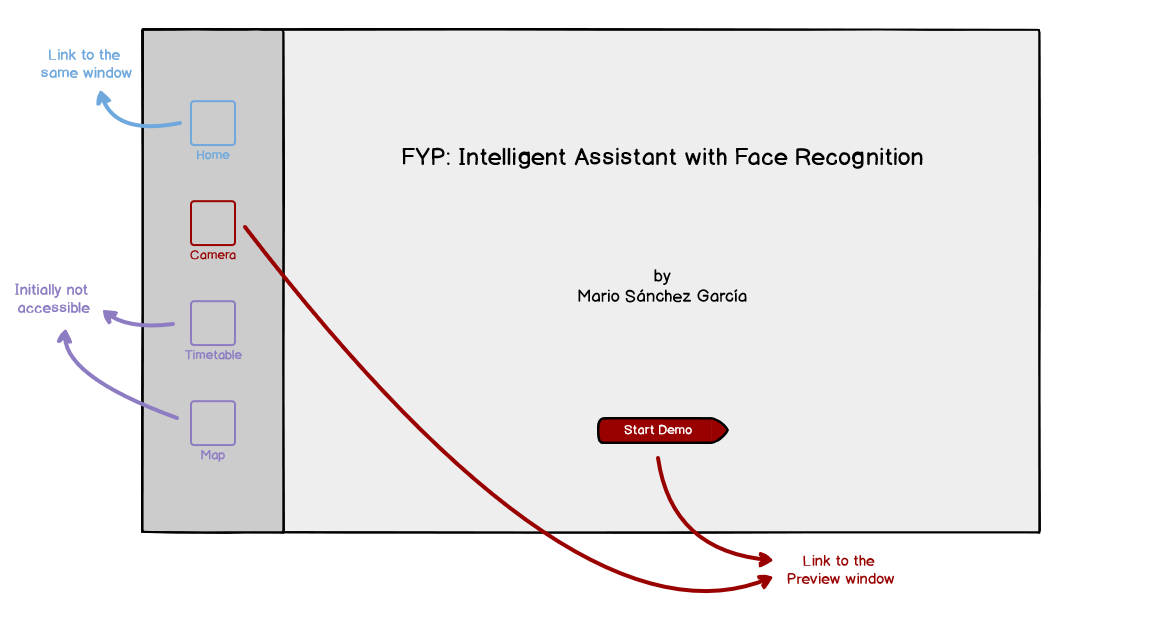
\includegraphics[width=15cm]{mockups/app_1_home_window.png}
		\caption{Home window of the application}
		\label{fig:home_window}
	\end{figure}

	\subsection{Preview window}
	\label{subsec:preview_window}

	This window (Figure \ref{fig:preview_window}) shows the a real time video stream of the camera, which will allow the users to have time to position themselves in front of the camera. In the lateral menu, the first icon links to the Home window (\ref{subsec:home_window}) and if it is clicked, the Home window will show up. The second links to this same window. The last two icons are disabled but still visible for the same reason of the previous window (the data needed to fill this windows has not been obtained yet).

	\begin{figure}[!ht]
		\centering
		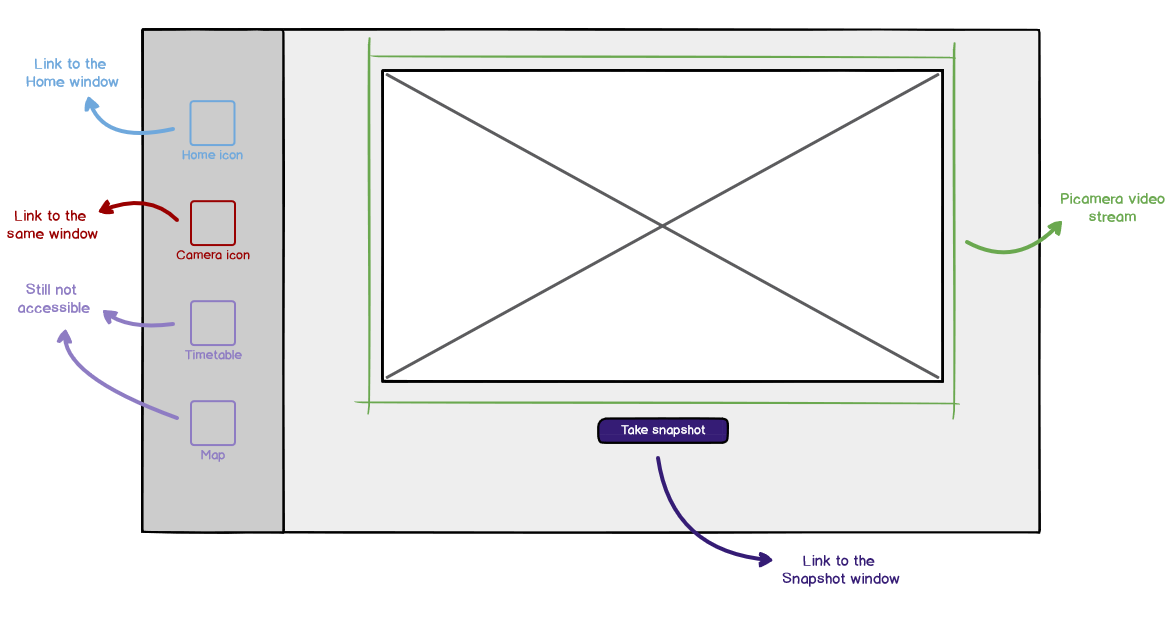
\includegraphics[width=15cm]{mockups/app_2_preview_window.png}
		\caption{Preview window of the application}
		\label{fig:preview_window}
	\end{figure}

	In the main panel of the right, the video stream of the \gls{picamera} is shown. The images of the stream have been flipped 180 degrees, as the camera is upside-down, and horizontally mirrored, so if the user moves to the right, the movement will be to the right in the preview as well. The button below the preview links to the Snapshot window (\ref{subsec:snapshot_window}) and will take the current video frame as the selected image in the moment it is clicked.

	\subsection{Snapshot window}
	\label{subsec:snapshot_window}
	This window (Figure \ref{fig:snap_window}) shows the image that was selected previously and that we will call \textit{\gls{snapshot}}. In the lateral menu, the first icon links to the Home window (\ref{subsec:home_window}) and if it is clicked, the Home window will show up. The second icon and the button "Take another snapshot" has the same action: show again the Preview window (\ref{subsec:preview_window}) and discard the current snapshot. The last two icons are disabled but still visible for the same reason of the Home window (the data needed to fill this windows has not been obtained yet).

	\begin{figure}[!ht]
		\centering
		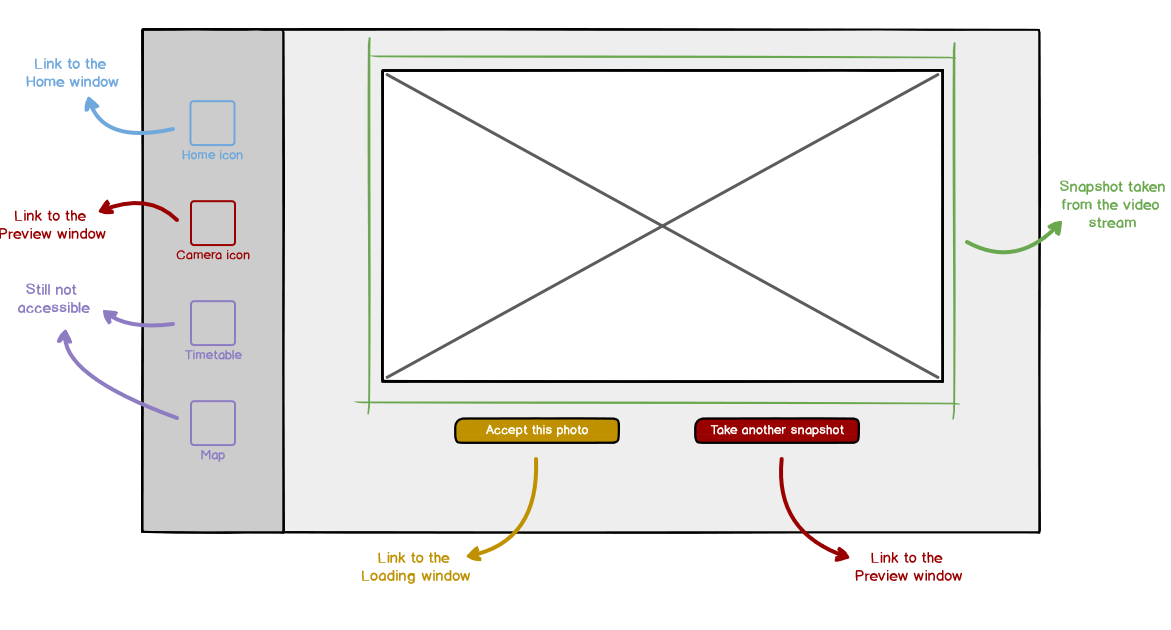
\includegraphics[width=15cm]{mockups/app_3_snap_window.png}
		\caption{Snapshot window of the application}
		\label{fig:snap_window}
	\end{figure}

	In the main panel of the right we can see the snapshot selected in the Preview window. The "Accept this photo" button links with the Loading window (\ref{subsec:loading_window}) and will send the snapshot to the server in order to identify the user as a student.

	\subsection{Loading window}
	\label{subsec:loading_window}
	This window (Figure \ref{fig:loading_window}) shows the progress in the communication with the server. All icons of the lateral menu will be disabled until the communication with the server is over. Depending of the call of the server that is being used at the moment, some icons of the menu will be different:

	\begin{itemize}
		\item Face recognition. The timetable icon will represent an user and it will be blinking each 0.5 seconds, being black in one phase and yellow in the other. 
		\item Get next class. The timetable icon will represent a calendar and it will be blinking each 0.5 seconds, being black in one phase and yellow in the other.
		\item Get map. The map icon will represent a map pin and it will be blinking each 0.5 seconds, being black in one phase and yellow in the other.
	\end{itemize}

	\begin{figure}[!ht]
		\centering
		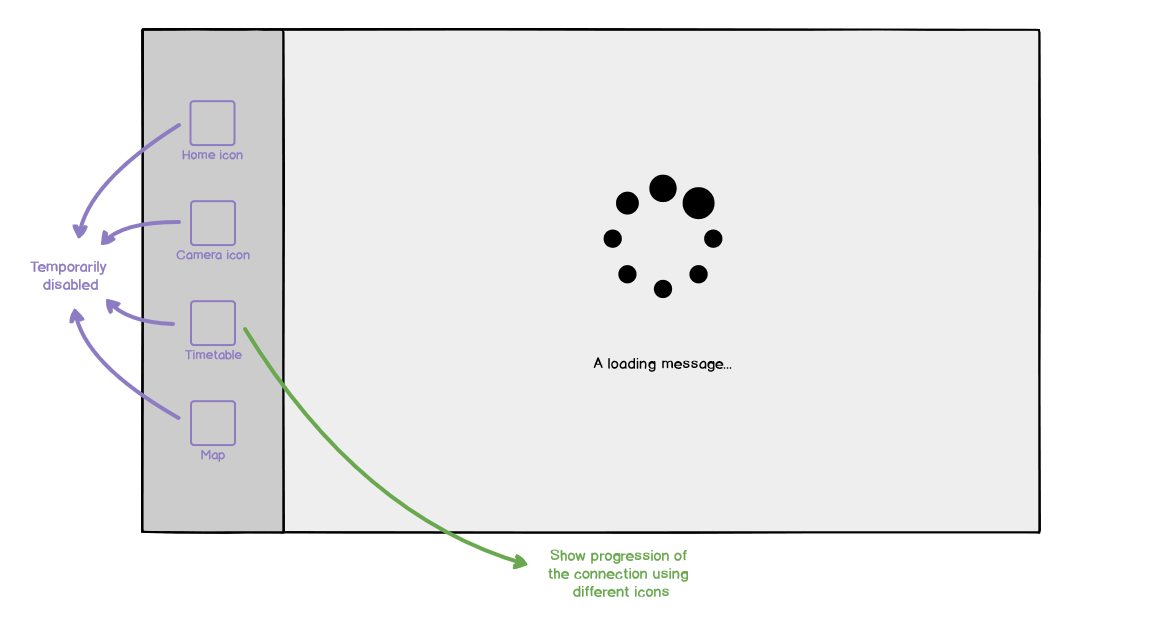
\includegraphics[width=15cm]{mockups/app_4_loading_window.png}
		\caption{Loading window of the application}
		\label{fig:loading_window}
	\end{figure}

	The snapshot from the previous window is sent to the server using a HTTP POST method to the route that it has for the face recognition service. The image is coded as UNICODE characters, so is can be wrapped using JSON. The server extracts the image from the request and decodes the JSON message to obtain again the original image. The server now applies the face detection proccess, where the faces detected are cropped out from the original image and saved in a new file. Now there are three possibilities depending of the output of this process (Figure \ref{fig:output_face_det}).

	\begin{figure}[!ht]
		\centering
		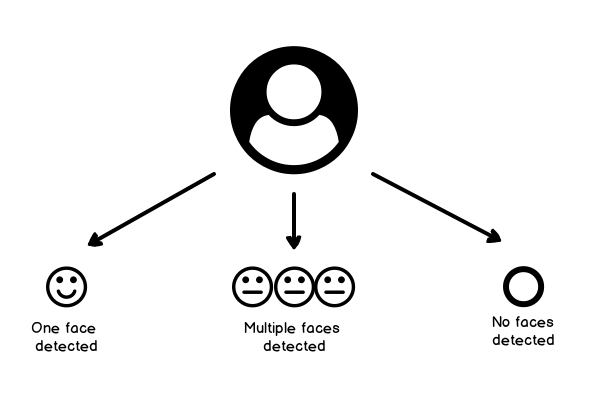
\includegraphics[width=9cm]{output_face_det.png}
		\caption{Possible outputs of the Face Detection process}
		\label{fig:output_face_det}
	\end{figure}

	The first possibility is that only one face is detected, which is the expected output of this process, being this face the one selected for the face recognition process. Another is that more than one face is detected, but in this case the first and leftmost face detected is the one selected for the face recognition process. The third and last possibility is that no faces are detected in the original image. Under these circumstances the server will send back a predefined default student instance along with a flag that will report the Raspberri Pi that no face could be detected. The Raspberry Pi will then show the Error window (\ref{subsec:error_window}) with a message informing the user about the situation.

	Following the expected output of the face detection process where only one face is detected, the face recognition process is applied to the new file with the cropped face. It will give back the student ID number of the recognised student with highest confidency percenteage (how sure is the \gls{cnn} of that the student in front of the camera is the recognised student) and the actual value of this confidency percenteage. 

	\begin{figure}[!ht]
		\centering
		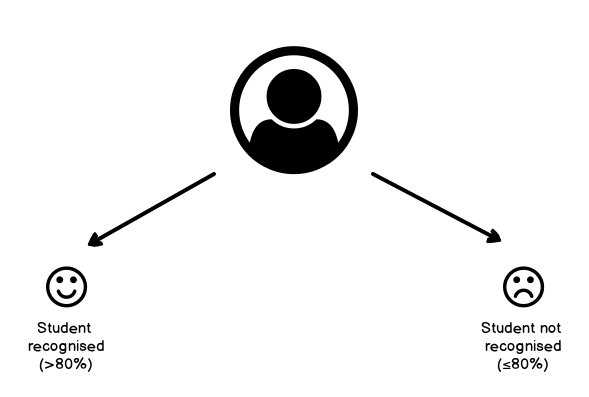
\includegraphics[width=9cm]{output_face_recog.png}
		\caption{Possible outputs of the Face Recognition process}
		\label{fig:output_face_recog}
	\end{figure}

	If the percenteage is less than 80\%, we will assume that the student is not recognised and therefore that the user is not a student. The system will follow a similar procedure to the no-face-detected case of before, but the flag sent will be different, informing that the student could not be detected. The Raspberry Pi will do the same as well, showing the Error window (\ref{subsec:error_window}) with a message to report the user about the situation. Otherwise, if the confidency percenteage is greater than 80\%, the server will take the name of the user from the database and send it along the ID number to the Raspberry Pi.

	Now that the Raspberry Pi knows the identity of the student, it will do another call to the server to get their next class of the day using the student's ID number. The server will use this ID to log into the timetable website of the University of Limerick (timetable.ul.ie). The website will give back as a response a static HTML page with a fixed pattern that contains the timetable. Analysing this pattern, the server will extract the timetable information from the fields of this HTML page and store it into a dictionary. Then, the current hour and weekday are taken into consideration to obtain the next class of the student.   

	\begin{figure}[!ht]
		\centering
		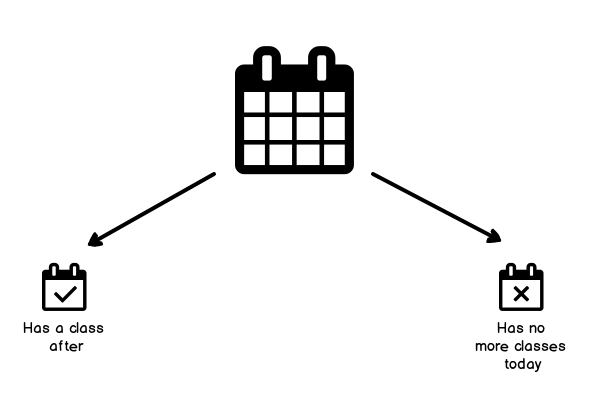
\includegraphics[width=9cm]{output_next_class.png}
		\caption{Possible outputs of the process of obtaining the next class}
		\label{fig:output_next_class}
	\end{figure}

	If the student has no more classes in the day or the last class of the day has already begun, a JSON is filled for the response with a null value (\textit{None} in Python) and sent back. In this situation, the Raspberry Pi will show the No More Classes window (\ref{subsec:no_classes}) to inform the student about the situation. On the other hand, if the student actually has a next class, the previous referred JSON would be filled with the data of this class, which include: code of the module, name of the module, starting hour, ending hour, class type and location of the classroom.

	Finally, the Raspberry will use the class information to obtain the map from the server. The current location of the student and the location of the classroom, formatted as latitude and longitude coordinates, are sent to the server using the specific route for the map. The server will receive these locations and use them to construct first a link to obtain the path from one point to the other, and then another link to obtain the map image. This image is sent back to the Raspberry Pi, that uses all the gathered information to fill the Timetable (\ref{subsec:timetable_window}) and Map (\ref{subsec:map_window}) windows.

	Once the communication with the server is over and the windows have been updated, the application shows the Timetable window automatically.

	\subsection{Timetable window}
	\label{subsec:timetable_window}
	This window (Figure \ref{fig:timetable_window}) shows the a welcome message using the name of the recognised student and some information of the next class of this student, such as the code and name of the module, the location and the type of class. In the lateral menu now all icons are available. These icons are Home (\ref{subsec:home_window}), Camera (\ref{subsec:preview_window}), Timetable and Map. The last icon has the same function as the button that is placed in the main panel of the right, which is to link this window to the Map window (\ref{subsec:map_window}). 

	\begin{figure}[!ht]
		\centering
		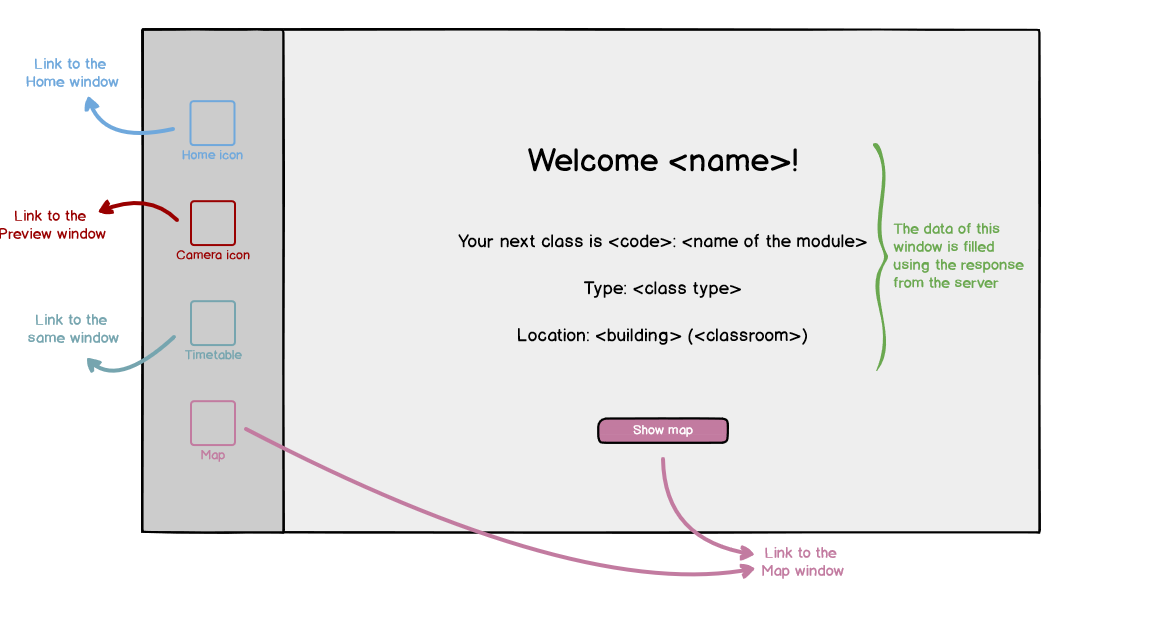
\includegraphics[width=15cm]{mockups/app_5_timetable_window.png}
		\caption{Timetable window of the application}
		\label{fig:timetable_window}
	\end{figure}

	\subsection{Map window}
	\label{subsec:map_window}
	This window (Figure \ref{fig:map_window}) shows the map to the next class of the student. In the lateral menu all icons are available. These buttons are These icons are Home (\ref{subsec:home_window}), Camera (\ref{subsec:preview_window}), Timetable (\ref{subsec:timetable_window}) and Map. In the top of the main panel of the right we can find the code and name of the module of the next class. Below it, the map image is displayed in a \gls{720p} resolution.

	\begin{figure}[!ht]
		\centering
		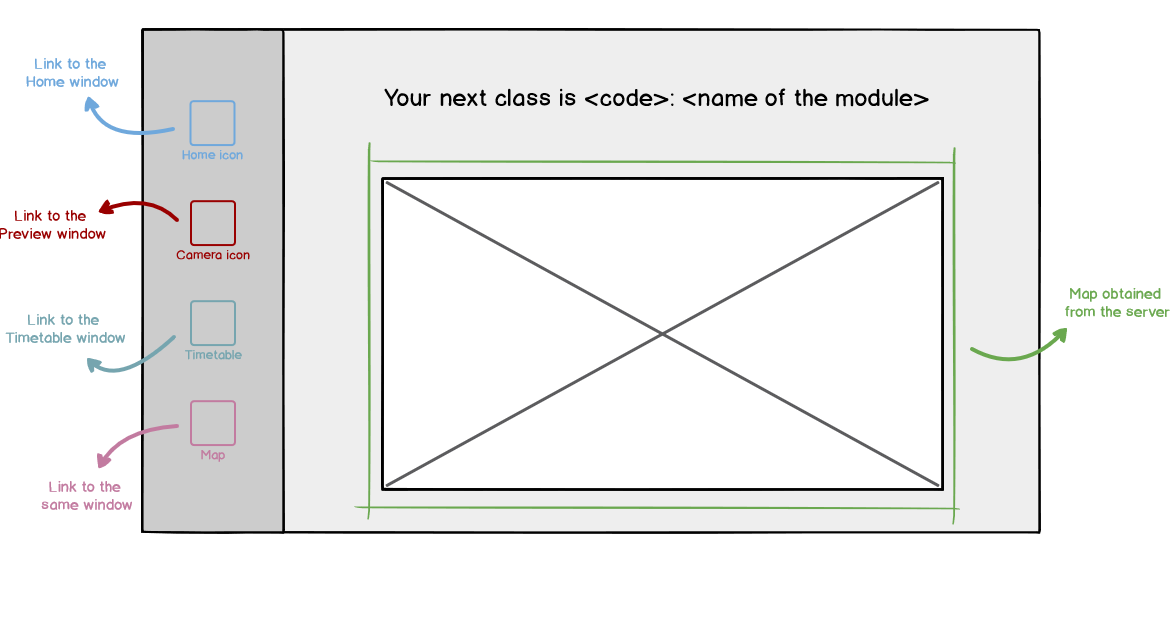
\includegraphics[width=15cm]{mockups/app_6_map_window.png}
		\caption{Map window of the application}
		\label{fig:map_window}
	\end{figure}

	\subsection{Error window}
	\label{subsec:error_window}
	This window (\ref{fig:error_window}) shows the user the kind of error that has occurred to the application. Only two possible errors are handled: \textit{no faces could be detected in the taken snapshot} or \textit{the user could not be identified as a student of the University of Limerick}. In both cases a message informing about the situation is displayed below a red cross icon in the main panel. 

	\begin{figure}[!ht]
		\centering
		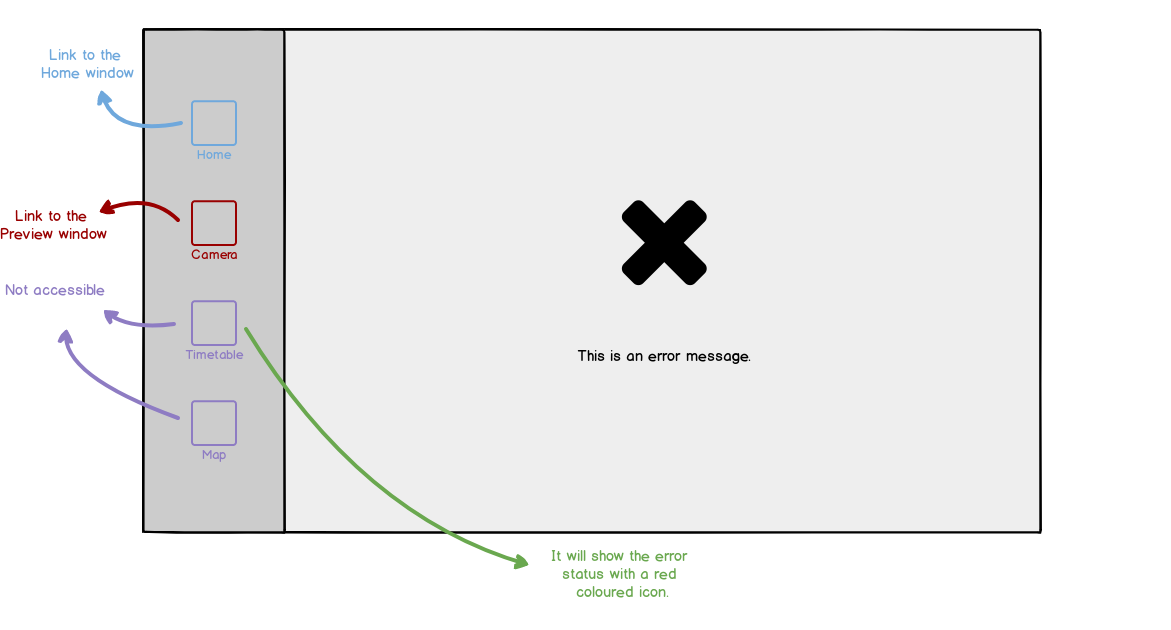
\includegraphics[width=15cm]{mockups/app_x_error_window}
		\caption{Error window of the application}
		\label{fig:error_window}
	\end{figure}	

	In the lateral menu we can find the Home and the Camera icons, that will link with the Home (\ref{subsec:home_window}) and Preview (\ref{subsec:preview_window}) windows, respectively. The third icon will represent a user using the red colourr instead of the usual Timetable icon and it will be disabled. When the user goes to another window from this point, this third icon will be still disabled but now showing the Timetable icon. The fourth and last icon will represent a Map pin, but as the map could not be obtained because of the error, it will be disabled.

	\subsection{No More Classes window}
	\label{subsec:no_classes}
	This window (\ref{fig:no_classes_window}) shows the user a welcome message using the name of the student and another message informing that the student has no more classes that day. In the lateral menu we can find the Home and the Camera icons, that will link with the Home (\ref{subsec:home_window}) and Preview (\ref{subsec:preview_window}) windows, respectively. The third will be the Timetable icon and in this case it will be not disabled.
	% When the user goes to another window from this point, this third icon will become disabled with the same icon.
	The fourth and last icon will represent a Map pin, but as the map could not be obtained because the user has no more classes, it will be disabled.

	\begin{figure}[!ht]
		\centering
		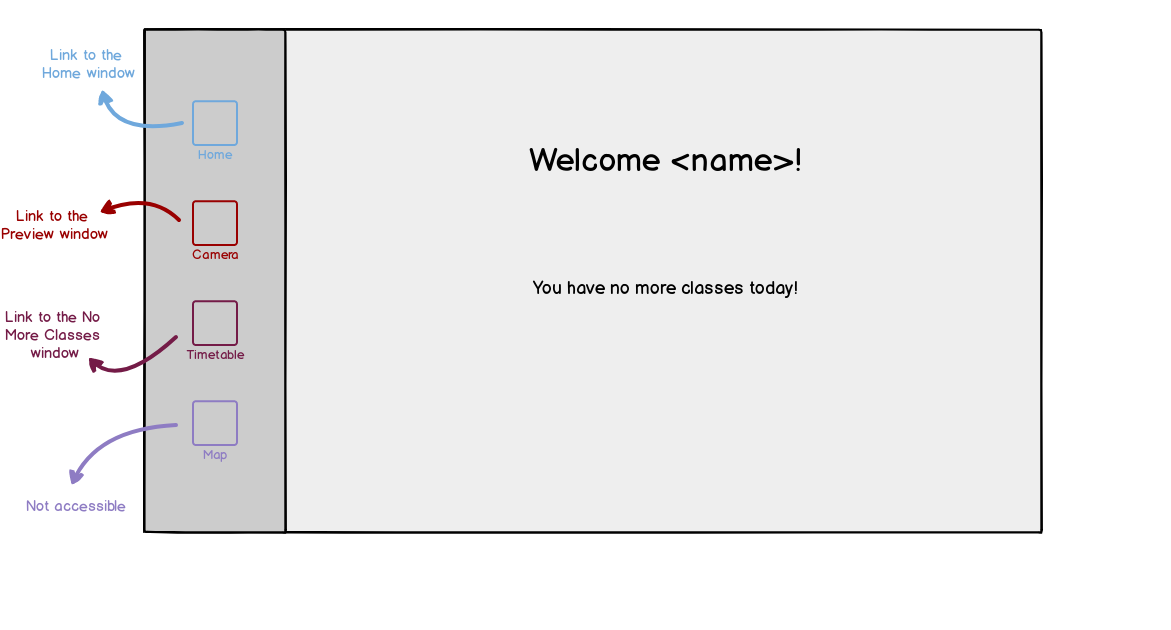
\includegraphics[width=15cm]{mockups/app_x_noclasses_window}
		\caption{No More Classes window of the application}
		\label{fig:no_classes_window}
	\end{figure}	



% █████╗ ██████╗  ██████╗██╗  ██╗██╗████████╗███████╗ ██████╗████████╗██╗   ██╗██████╗ ███████╗
%██╔══██╗██╔══██╗██╔════╝██║  ██║██║╚══██╔══╝██╔════╝██╔════╝╚══██╔══╝██║   ██║██╔══██╗██╔════╝
%███████║██████╔╝██║     ███████║██║   ██║   █████╗  ██║        ██║   ██║   ██║██████╔╝█████╗  
%██╔══██║██╔══██╗██║     ██╔══██║██║   ██║   ██╔══╝  ██║        ██║   ██║   ██║██╔══██╗██╔══╝  
%██║  ██║██║  ██║╚██████╗██║  ██║██║   ██║   ███████╗╚██████╗   ██║   ╚██████╔╝██║  ██║███████╗
%╚═╝  ╚═╝╚═╝  ╚═╝ ╚═════╝╚═╝  ╚═╝╚═╝   ╚═╝   ╚══════╝ ╚═════╝   ╚═╝    ╚═════╝ ╚═╝  ╚═╝╚══════╝
                                                                                              

\section{Architecture}
\label{sec:architecture}
In this project the architecture follows the pattern Model-View-Controller (\gls{mvc}). It was first described in the original MVC note at Xerox PARC in 1978, by the Norwegian computer scientist Trygve Reenskaug (\cite{mvc_origin}). The first name of the pattern was "Thing Model View Editor" (\cite{tmve_reenskaug_1979}), but he quickly changed it to the popular "Model View Controller" (\cite{mvc_reenskaug_1979}). This first version of MVC was first implemented as part of the Smalltalk-80 class library and originally used as an architectural pattern to create \glspl{gui}.

However, the definition of the MVC pattern has changed over the time to adapt to the changing environment. And because of this fact, it is one of the most quoted (and most misquoted) patterns around (\cite{current_mvc_definition}). A general and basic definition of the pattern is shared by most of the approaches and has been summarized in the Figure \ref{fig:mvc_diagram}.   

\begin{figure}[!ht]
	\centering
	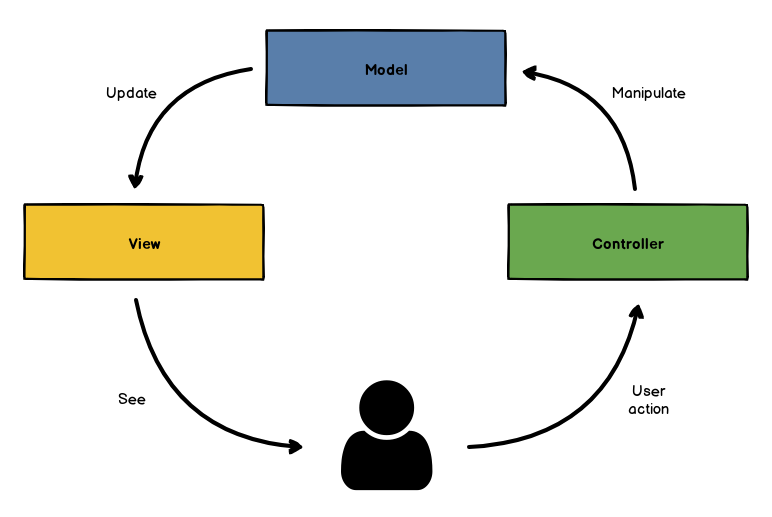
\includegraphics[width=10cm]{mvc_diagram.png}
	\caption{MVC pattern diagram}
	\label{fig:mvc_diagram}
\end{figure}	

It is a software architecture pattern that divides the system in three different components named Model, View and Controller: the application data, the user interface and the control logic, respectively (\cite{mvc_components_definition}).
\begin{itemize}
	\item Model. It is the information representation with which the system operates, managing every access to this information. The interaction with the other components consists in 	sending the information to the data to the View to be visualised by the user and accepting or denying the access and modifying requests that come from the Controller.
	\item View. It shows the Model in an appropiate format that allows users to interact with the system, usually using a \gls{gui}.
	\item Controller. It responds to the user actions and access the Model to query or modify the information contained in it. It also communicates with the View in order to apply the changes of the Model by the use of requests. 
\end{itemize}

In the high level context of this project, the View correspond to the Raspberry Pi application, the Controller is the server located at the laptop, and the Model is the database that the server queries to find the student's information. 

	\subsection{Back-end architecture}
	Unlike the Front End, which is contained in a single called "app.py", the Back End of the project is divided in multiple files/modules. The component diagrams have been included in the Figures \ref{fig:back_comp_diagram} and \ref{fig:face_recog_comp_diagram} to explain the interaction between these modules, 

	\clearpage

	\begin{figure}[!ht]
		\centering
		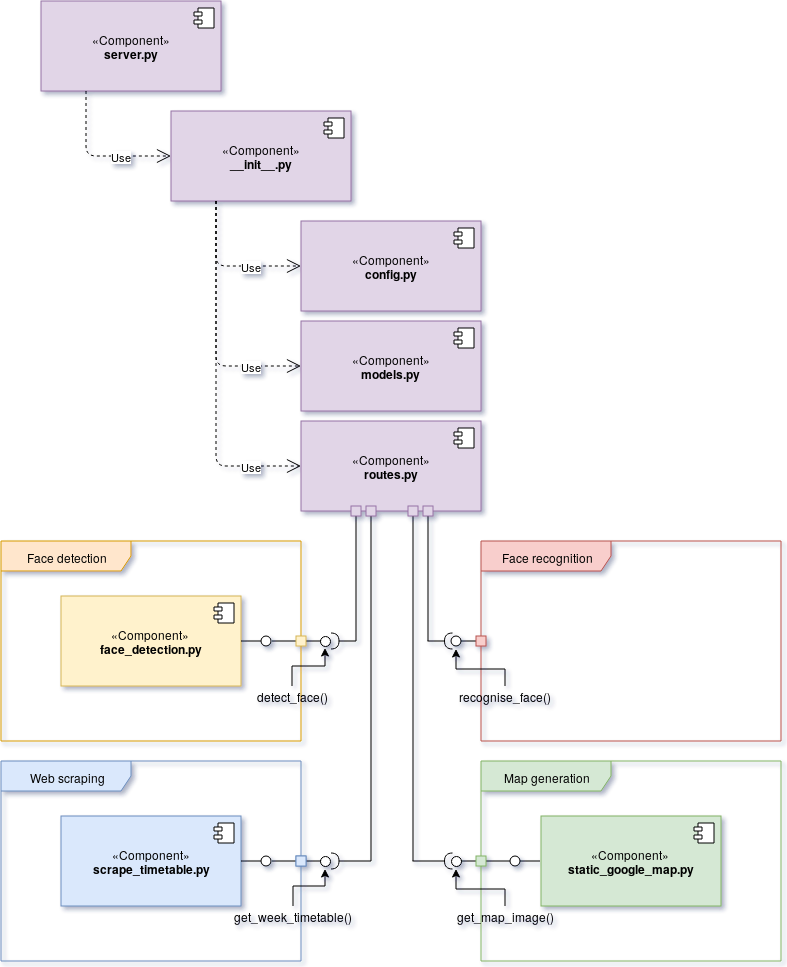
\includegraphics[width=14cm]{back-end_comp_diagram}
		\caption{Component diagram of the Back End of the system}
		\label{fig:back_comp_diagram}
	\end{figure}	

	\clearpage

	\begin{figure}[!ht]
		\centering
		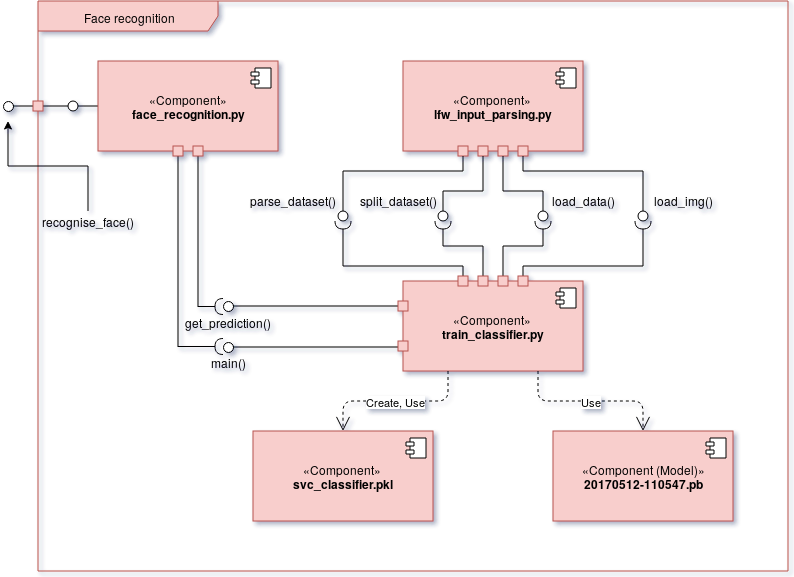
\includegraphics[width=14cm]{face-recog_module_comp_diagram}
		\caption{Component diagram of the Face recognition module}
		\label{fig:face_recog_comp_diagram}
	\end{figure}	



%████████╗███████╗ ██████╗██╗  ██╗███╗   ██╗ ██████╗ ██╗      ██████╗  ██████╗ ██╗███████╗███████╗
%╚══██╔══╝██╔════╝██╔════╝██║  ██║████╗  ██║██╔═══██╗██║     ██╔═══██╗██╔════╝ ██║██╔════╝██╔════╝
%   ██║   █████╗  ██║     ███████║██╔██╗ ██║██║   ██║██║     ██║   ██║██║  ███╗██║█████╗  ███████╗
%   ██║   ██╔══╝  ██║     ██╔══██║██║╚██╗██║██║   ██║██║     ██║   ██║██║   ██║██║██╔══╝  ╚════██║
%   ██║   ███████╗╚██████╗██║  ██║██║ ╚████║╚██████╔╝███████╗╚██████╔╝╚██████╔╝██║███████╗███████║
%   ╚═╝   ╚══════╝ ╚═════╝╚═╝  ╚═╝╚═╝  ╚═══╝ ╚═════╝ ╚══════╝ ╚═════╝  ╚═════╝ ╚═╝╚══════╝╚══════╝
                                                                                                 


\section{Technologies}
\label{sec:techs}
In the following sub-sections we will include all the technologies that have been used in the development of this project, also represented in the Marketecture diagram (Figure \ref{fig:marketecture_diagram}).

\begin{figure}[!ht]
	\centering
	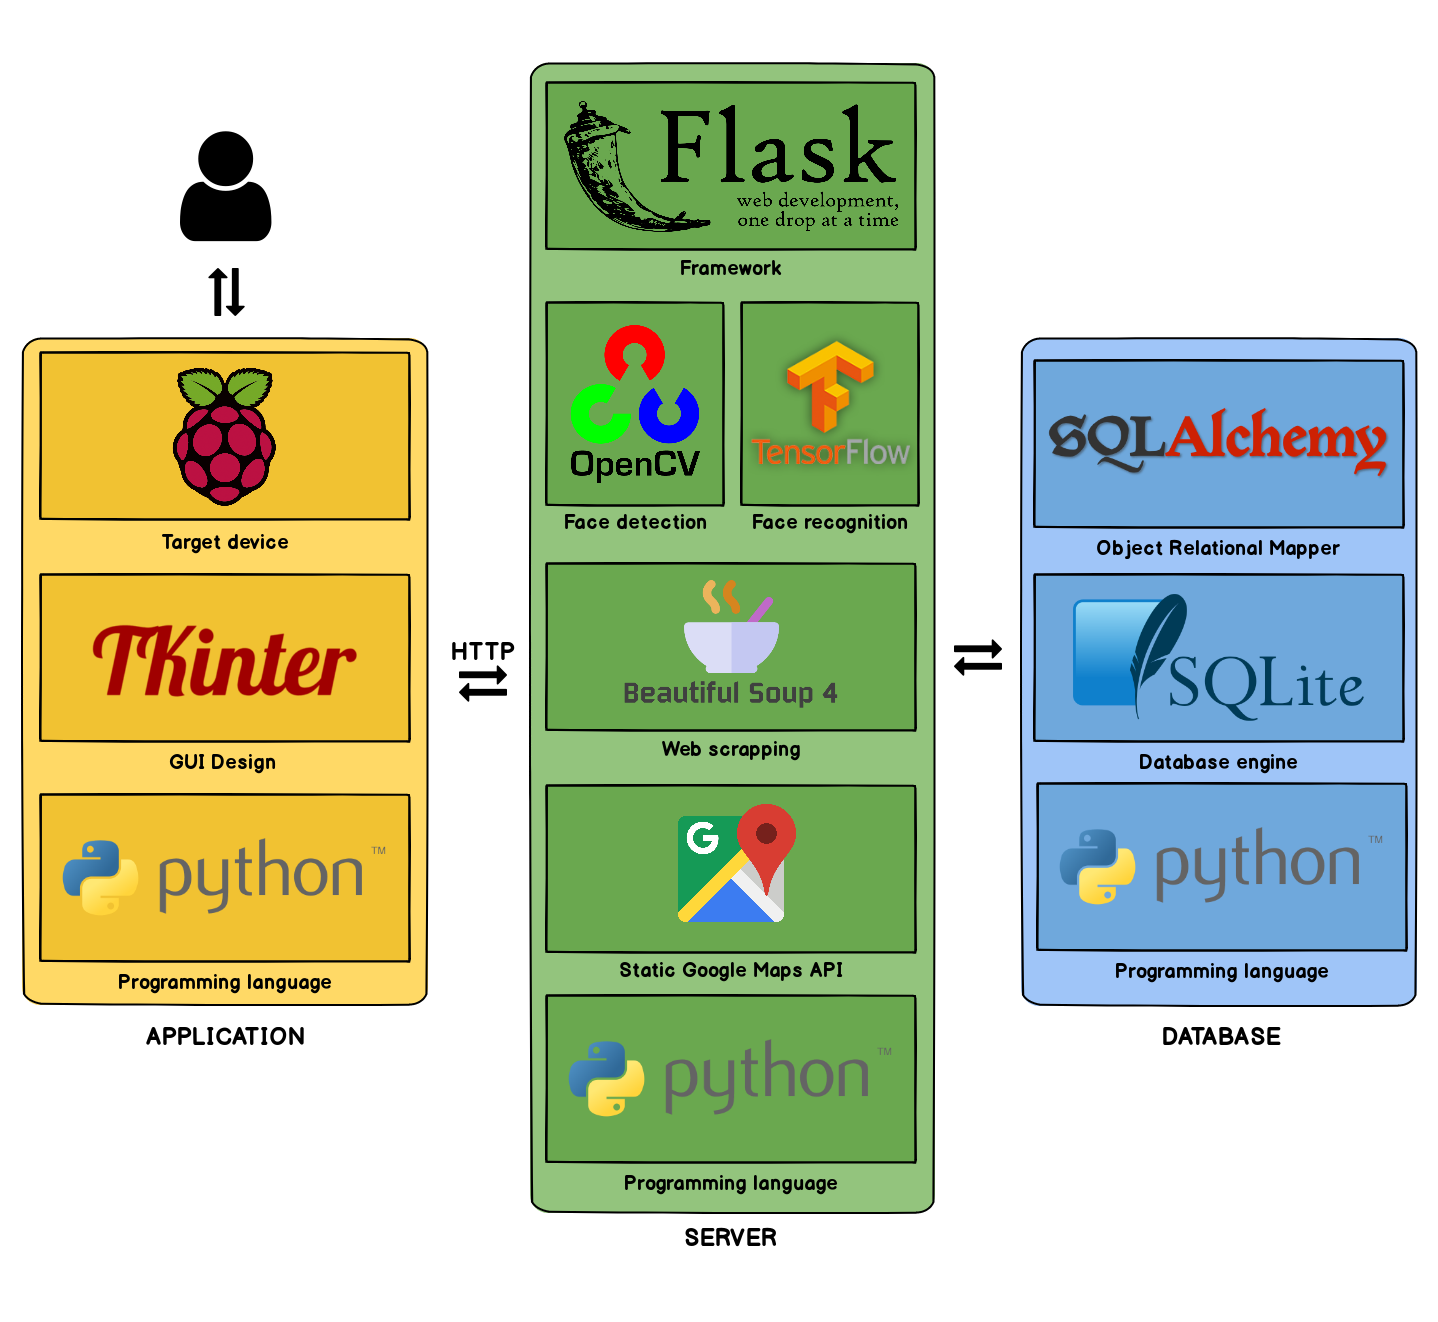
\includegraphics[width=14.5cm]{marketecture_diagram}
	\caption{Marketecture diagram}
	\label{fig:marketecture_diagram}
\end{figure}	

	\subsection{Python}
	Another section about this language was included in the Research, so here we will only talk about the decissions made about it, referring to \ref{sec:python} for all the background information. For the development of this project, the version 3.6.3 of Python was finally chosen over the 2.x or legacy. The main reason of this choice is that all recent standard library improvements are only available by default in Python 3.x (\cite{python_2or3}) and, eventually, there will be no future security or bug fixes for Python 2.x.

	One of the most popular problems when working with Python is the version of the dependencies, because one application may need the version 1 of a dependency, but another application requires version 2. To solve this problem, the \cite{virtualenv} tool was used to create isolated environments that have their own installation directories.  

	\subsection{Tensorflow}
	TensorFlow is an open source software library for high performance numerical computation. Its flexible architecture allows an easy deployment across a variety of platforms, such as desktop computers, clusters and mobiles devices. It was originally developed by researchers and engineers from the Google Brain team within Google’s AI organization (\cite{tensorflow_main_website}). It has a strong support for machine learning and deep learning processes, which is for what it will be used in this project. 

	\begin{figure}[!ht]
		\centering
		
\includegraphics[width=5cm]{logos/tensorflow.png}
		\caption{Tensorflow official logo (\cite{tensorflow_main_website})}
		\label{fig:tensorflow}
	\end{figure}

	The "CPU support only" type of Tensorflow was installed in the server machine for Python3. The creation of a \gls{cnn} model from scratch that would be actually capable to perform face recognition is outside the scope of a \gls{fyp}. Because of this reason, we chose a pre-trained model from the famous FaceNet project (\cite{facenet_article}) that uses the architecture Inception Resnet v1.

	Another possible architecture would have been Inception-v3. Both of them have been proven to give excellent results in image and face recognition, but as seen in \cite{inception_resnet_article}, with a similar computational cost, the training proccess of the Inception Resnet v1 is faster (Figure \ref{fig:incep_arch_diff}).

	\begin{figure}[!ht]
		\centering
		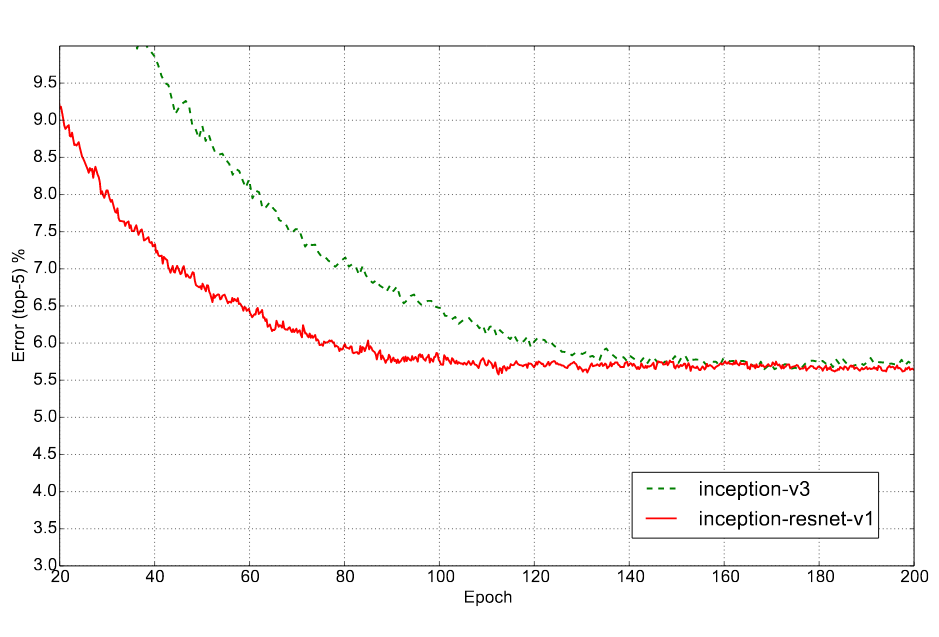
\includegraphics[width=10cm]{network_arch_diff.png}
		\caption{Top-5 error evolution during training of pure Inception-v3 vs Inception Resnet v1 (\cite{inception_resnet_article}))}
		\label{fig:incep_arch_diff}
	\end{figure}

	\subsection{OpenCV}
	\label{subsec:opencv}
	OpenCV (Open Source Computer Vision Library) is an open source computer vision and machine learning software library. OpenCV was built to provide a common infrastructure for computer vision applications and to accelerate the use of machine perception in the commercial products. Being a BSD-licensed product, OpenCV is free for comercial and personal use and allow to modify the code (\cite{opencv_about}). It has C++, Python, Java and MATLAB interfaces and supports Windows, Linux, Android and Mac OS, so the Python interface for Linux was chosen for this project. 

	\begin{figure}[!ht]
		\centering
		\vspace{0.2cm}
		
\includegraphics[width=4cm]{logos/opencv.png}
		\caption{OpenCV official logo (\cite{opencv_about})}
		\label{fig:opencv}
	\end{figure}	

	In the server, this library has been used to pre-process the image captured in the Raspberry Pi before feeding it to the trained network. A face detection process using the Viola-Jones method (Haar-Cascade) is applied on this image, cropping the face out to a new file. 

	It has become also really popular outside the computer vision and machine learning environment thanks to its image processing functions, which is for what is mainly used in the Raspberry Pi. However, this library is only installed by default in the Raspberry Pi for Python 2.x. In order to install it for the Python 3, the tutorial in \cite{opencv_for_python3} was followed, where the author guide step-by-step through the compile and installation process.

	\subsection{Flask Server}
	Flask is an open-source microframework written in Python based on the Werkzeug toolkit and the Jinja 2 template engine. Like OpenCV, it is distributed under a BSD license, so it is free for comercial and personal use (\cite{flask_server_docs}). The communication with the server will be done using HTTP requests, wrapping the data of these requests in JSON format.

	\begin{figure}[!ht]
		\centering
		%\vspace{0.2cm}
		
\includegraphics[width=8cm]{logos/flask.png}
		\caption{Flask Server official logo (\cite{flask_server_docs})}
		\label{fig:flask_server}
	\end{figure}	

	This framework allow the developers to contain their application in a unique Python file. However, when the application starts to grow it the code becomes more difficult to maintain. Because of this reason, the server application has been divided in different files in a structure similar to the Figure \ref{fig:flask_files_struct}. The "server.py" file is the main file which is executed to run the server, "config.py" contains some configuration values that are applied in the context of the server application and "routes.py" has the different possible calls that the server has configured. The "{\_}{\_}init{\_}{\_}.py" file is the one that links these files and actually launch the flask application.

	\begin{figure}[!ht]
		\centering
		%\vspace{0.2cm}
		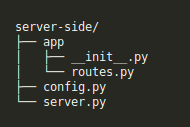
\includegraphics[width=4cm]{flask_files_structure.png}
		\caption{File structure in a Flask project}
		\label{fig:flask_files_struct}
	\end{figure}		

	\subsection{SQLAlchemy}
	\label{subsec:sql_alchemy}
	SQLAlchemy is a Python SQL toolkit and Object Relational Mapper (\gls{orm}) (\cite{sqlalchemy_main_website}). \glspl{orm} allow applications to manage a database using high-level entities such as classes, objects and methods instead of tables and SQL. This way, the developers can change the database engine of their application without having to change the code of the application. 

	\begin{figure}[!ht]
		\centering
		%\vspace{0.2cm}
		
\includegraphics[width=8cm]{logos/sqlalchemy.png}
		\caption{SQLAlchemy official logo (\cite{sqlalchemy_main_website})}
		\label{fig:sqlalchemy}
	\end{figure}

	For this project we have chosen the SQLite engine , which stores the databases as files on disk. The reason to choose it is that SQLite is really convenient for small applications with a single thread such as ours, as there is no need to run a database server like MySQL. The database schema used in the server is very simple (Figure \ref{fig:database_diagram}). It only has one table, Student, which stores the ID number and the name of the students recognised by the system. The database is filled with the student names and ID nummbers before running the server, executing the file \textit{reset{\_}db.py}.

	\begin{figure}[!ht]
		\centering
		%\vspace{0.2cm}
		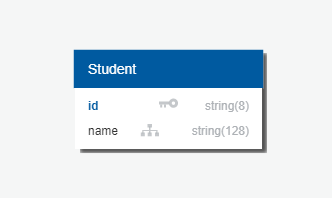
\includegraphics[width=8cm]{database_diagram.png}
		\caption{Database diagram of the system}
		\label{fig:database_diagram}
	\end{figure}

	\subsection{Tkinter} 
	Python provides several different libraries to create \glspl{gui}, being Tkinter one of the most widely known. It is the standard Python interface to the Tk \gls{gui} toolkit and provides cross-platform support (\cite{tkinter_docs}). It is also quite easy to use, although it does not have graphical editors, such as the ones existing for Java GUI developers. It was the library used to design the \gls{gui} of the Raspberry Pi application.  

	\subsection{Beautiful Soup}
	Beautiful Soup is a Python library designed for parsing HTML and XML documents that may have irregular markup, hence the name Beatiful "Soup" (\cite{beautiful_soup_main}). The parsed document is stored in a structure that can be used to extract data from these documents, practice known as web scraping if the document was in fact a website. In the project, the version 4.6 of this library it is used with this same purpose, extracting the student's timetable. 	

	\subsection{Google Static Maps API}
	The Google Static Maps API allow the developers to obtain a Google Maps image without requiring to use JavaScript or to render HTML. This service creates a map based on URL parameters sent through a standard HTTP request and returns the map as an image \cite{google_maps_static}. To use Google Maps APIs, developers must a register their project on the Google API Console in order to get a Google API key. Once obtained, every call to the API must include this key.

	Other Google Maps APIs also allow developers to use maps in their projects. However, the easiest way found to insert a map in a tkinter \gls{gui} was to use an image. This fact, along with the API's simple HTTP interface, made us to finally choose it for the project.

	\begin{figure}[!ht]
		\centering
		
\includegraphics[width=4.5cm]{logos/google_maps.png}
		\caption{Google Maps official logo (\cite{google_maps_static})}
		\label{fig:google_maps}
	\end{figure}

	\subsection{Latex}
	\LaTeX{} is a document preparation system for high-quality typesetting. It is most often used for medium-to-large technical or scientific documents but it can be used for almost any form of publishing (\cite{latex_main}). To generate a document using LaTeX, the process typically consists of using a text editor to edit the LaTeX source file (.tex), and then running LaTeX to convert this file to a format such as PDF.

	For someone familiar with MS Word or such word processors, the aspect of Latex that may stands out most is that there does not have to be an interaction with a \gls{gui} or that the document will not be as it looks like in the LaTeX file. However, it has many advantages such as its compatibility with version control or an excellent mathematical typesetting, reasons for what it was finally chosen for the project.

	\subsection{Version Control: Git}
	Git is a free and open source distributed version control system designed to handle everything from small to very large projects with speed and efficiency \cite{git_about}. Nowadays, Git, along with the web-based hosting service platform GitHub, have become very popular. In 2014, the Eclipse Foundation reported in its annual community survey that Git was at that moment the most widely used source-code management tool (\cite{git_popular}). 

	A private repository was created in Github to hold the project and Git was used to upload the diary changes to the platform. The structure of this repository (Figure \ref{fig:github_project_structure}) is divided in:

	\begin{itemize}
		\item \textit{.git}. Folder that contains all the files related to the Git version control management of the project.
		\item \textit{pi-assistant}. It contains the source code of the application and the server, organised in the subfolders "pi-side" and "server-side", respectively.
		\item \textit{report}. It contains the .tex files of this report, along with all images used here and the final PDF version.
		\item \textit{utils}. This folder contains the source code previous work, done in order to develop the different functionalities of the server side. 
		\item \textit{.gitignore}. File that allows to ignore (hence its name) certain files or extensions when the changes are committed (registered).
		\ item \textit{README.md}. File that contains the abstract of the project in markdown language, which is loaded and shown as text in the Github website. 
	\end{itemize}

	\begin{figure}[!ht]
		\centering
		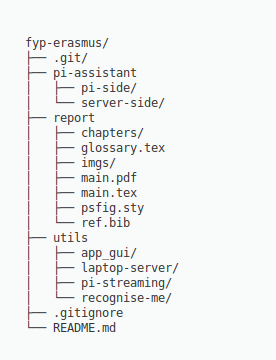
\includegraphics[width=4.5cm]{github_project_structure}
		\caption{Github project structure}
		\label{fig:github_project_structure}
	\end{figure}


%███████╗██████╗  ██████╗ ███╗   ██╗████████╗    ███████╗███╗   ██╗██████╗ 
%██╔════╝██╔══██╗██╔═══██╗████╗  ██║╚══██╔══╝    ██╔════╝████╗  ██║██╔══██╗
%█████╗  ██████╔╝██║   ██║██╔██╗ ██║   ██║       █████╗  ██╔██╗ ██║██║  ██║
%██╔══╝  ██╔══██╗██║   ██║██║╚██╗██║   ██║       ██╔══╝  ██║╚██╗██║██║  ██║
%██║     ██║  ██║╚██████╔╝██║ ╚████║   ██║       ███████╗██║ ╚████║██████╔╝
%╚═╝     ╚═╝  ╚═╝ ╚═════╝ ╚═╝  ╚═══╝   ╚═╝       ╚══════╝╚═╝  ╚═══╝╚═════╝ 

\section{Front end}
\label{sec:front_end}
This section includes some captures of fragments of code from the front-end side of the system. Using these captures, a brief explanation of how this code work is also given. The front-end of the system is all contained in the "app.py" file, that creates and launchs the \gls{gui}.

The library \textit{tkinter} (not \textit{Tkinter}, which is for Python 2.x) is imported along with its module "ttk". Some names are defined in both libraries and at the time of reading the code, it may be not clear which library is being used. In order to make the code clearer, the global import has been avoided (Figure \ref{fig:import_tkinter}). 

\begin{figure}[!ht]
	\centering
	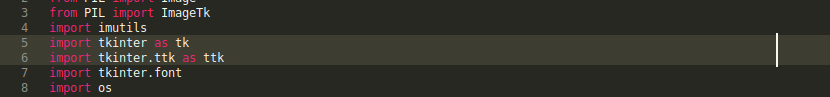
\includegraphics[width=14cm]{front_captures/tk_explicit}
	\caption{Importing tkinter}
	\label{fig:import_tkinter}
\end{figure}

As we can see in the Figure \ref{fig:class_and_main}, the tkinter application is inside the \textit{FullScreenApp} class. An instance of this class is created in the main function, taking as parameters the IP direction of the server and the image directory from where icons and images will be loaded. After, the main loop of the GUI starts, waiting for the user inputs to the application. 

\begin{figure}[!ht]
	\centering
	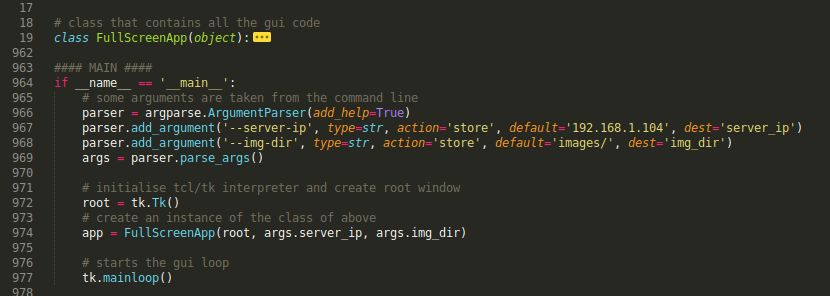
\includegraphics[width=14cm]{front_captures/class_and_main}
	\caption{Main function and class header}
	\label{fig:class_and_main}
\end{figure}

In the moment the instance of the class is created, the {\_\_}init{\_\_} function is called, taking the parameters and storing them in the \textit{self} object (Figure \ref{fig:init_head}). The video stream thread of the \gls{picamera} is launched using the \textit{imutils} library, and the master window is configured to be displayed in fullscreen. Although the video stream is not displayed for now, the picamera needs some warm-up time to work properly, so it is launched now with the purpose of having the picamera ready for when it will be required. 

\begin{figure}[!ht]
	\centering
	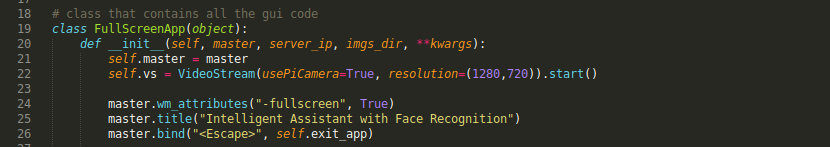
\includegraphics[width=14cm]{front_captures/init_f_header}
	\caption{{\_\_}init{\_\_} function}
	\label{fig:init_head}
\end{figure}

Three frames are attached to the master window (Figure \ref{fig:master_frames}): the lateral menu (\textit{navigation{\_}toolbar} in the code), the main panel of the right that will act as a container of the rest of the windows, and a last frame with the sole purpose of dividing the first two, hence its name \textit{line}.

\begin{figure}[!ht]
	\centering
	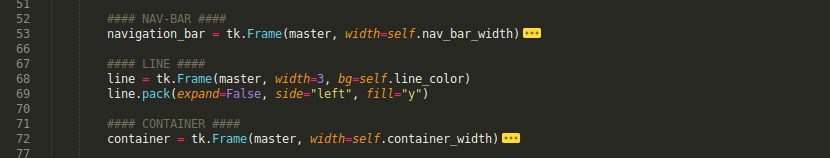
\includegraphics[width=14cm]{front_captures/master_frames}
	\caption{Creation of the frames attached to the master window}
	\label{fig:master_frames}
\end{figure}

Now the container's windows are created (Figure \ref{fig:container_frames}). The Frame objects are stored in the dictionary \textit{frames} of the \textit{self} object, so they will be accessible from anywhere inside the class. Then, the functions to create the contents of these frames are called (e.g. \textit{create{\_}home{\_}frame}).

\begin{figure}[!ht]
	\centering
	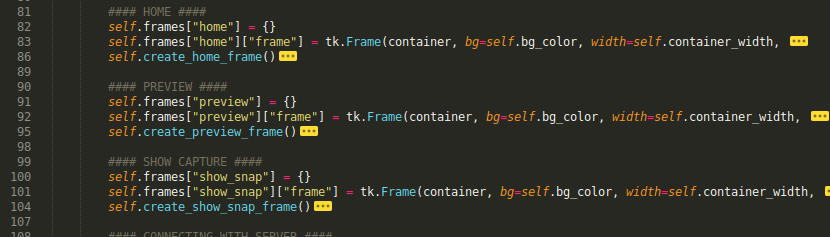
\includegraphics[width=14cm]{front_captures/container_frames}
	\caption{Creation of the frames attached to the container window}
	\label{fig:container_frames}
\end{figure}

Once all contents are created, the application shows the Home window, moment in which the function \textit{update{\_}nav{\_}bt} is called (Figure \ref{fig:update_nav_function}). This function is used to update the icons of the lateral menu. The logic used to decide which icon should be loaded is based in the evaluation of flags related to the container's frames. During the creation of each frame, flags such as \textit{is{\_}focus} were added to the \textit{frames} dictionary, so they can be accessed in the \textit{update{\_}nav{\_}bt} function. In this case, a "focused" frame will lead to change the colour of the icon representing this frame to blue. 

\begin{figure}[!ht]
	\centering
	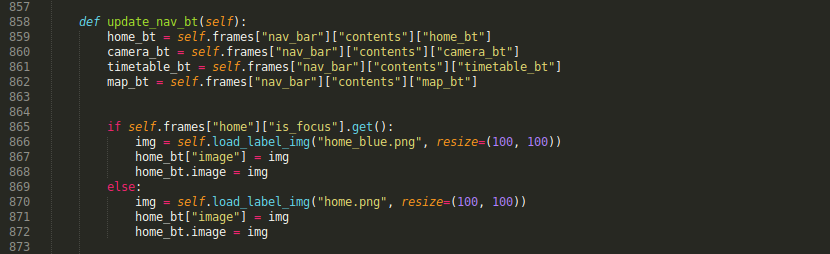
\includegraphics[width=14cm]{front_captures/update_nav_function}
	\caption{Updating the lateral menu icons}
	\label{fig:update_nav_function}
\end{figure}

Eventually, the user will press the start button of the Home window, showing the Preview window. The method followed to show the video stream inside the \gls{gui} was to get the current frame from the \textit{VideoStream} declared at the beginning and update the image shown in the frame. This process is contained in the \textit{video{\_}stream{\_}loop} function and is controlled by the flag \textit{stop{\_}video{\_}stream} (Figure \ref{fig:video_loop_function}).  

\begin{figure}[!ht]
	\centering
	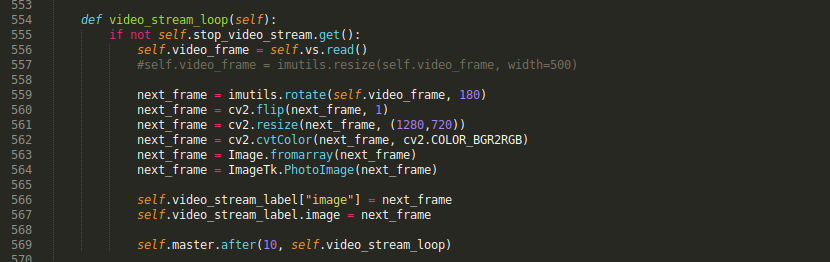
\includegraphics[width=14cm]{front_captures/video_loop}
	\caption{\textit{video{\_}stream{\_}loop} function}
	\label{fig:video_loop_function}
\end{figure}

The loop is created using the tkinter function \textit{after}, that allows the function to call itself after a certain amount of time (i.e. recursion). The reason to stop the video is that the Raspberry is a very limited device, so a heavy process like this uses most of its computational power. This can be proven by running the application, where the video stream shown on the screen does not even reach 30 \gls{fps} (the minimum callback time is set to 10ms, so it is theoretically possible). As said before, the recursion depends on the value of the flag:

\begin{itemize}
	\item \textit{false}. Starts the video stream. The flag is set to this value everytime the "focus" is passed to the Preview window.
	\item \textit{true}. Stops the video stream. The flag is set to this value everytime the "focus" is passed to another window, if the previous window was the Preview window.
\end{itemize}

When the user finally accept a snapshot, the connection with the server starts. A total of three phases are necessary to get all the data to fill the next windows of the application: recognise the student, get the next class and get the map to that class. Each phase is a call to the server, and as such, it will take some time to receive the response.

The tkinter function \textit{wait{\_}variable} is used to wait for the server response (Figure \ref{fig:connect_with_server}). First, a thread executing a function that sends the request to the server (i.e. auxiliary function) is launched and then the \textit{wait{\_}variable} function blocks the elements of the \gls{gui}. Once the server sends back a response, the auxiliary function updates the variable for what the \textit{wait{\_}variable} function is waiting, unlocking the flow of the application. 

In addition to the connection with the server itself, the \textit{connect{\_}with{\_}server} function also decides which is the frame to show depending of the responses of the server. In the auxiliary functions, other flags besides the one waited by \textit{wait{\_}variable} are set as well (e.g. \textit{is{\_}detected}). And it is through the use of these flags how the \textit{connect{\_}with{\_}server} function decides whether to show one frame or another. 

\begin{figure}[!ht]
	\centering
	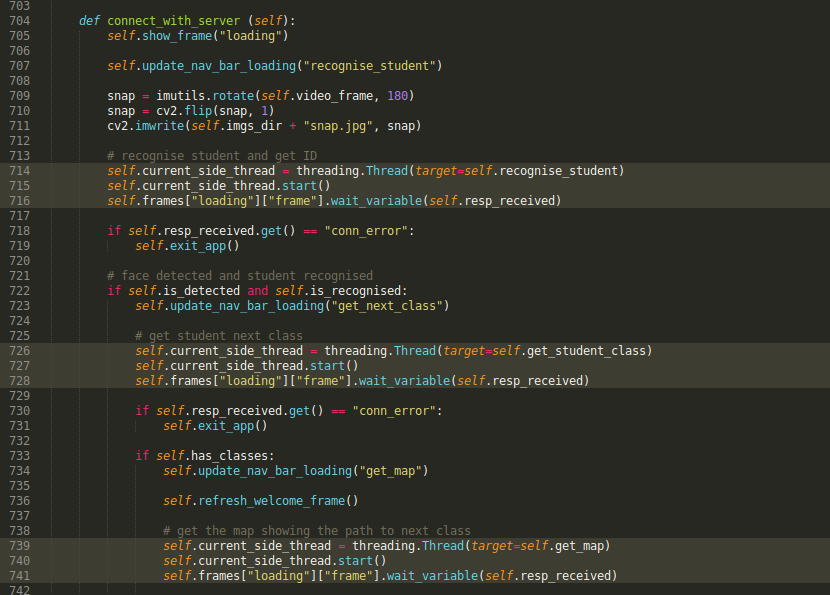
\includegraphics[width=14cm]{front_captures/connect_with_server}
	\caption{\textit{connect{\_}with{\_}server} function}
	\label{fig:connect_with_server}
\end{figure}

After this, the only thing left to do is to refresh the contents of the frames that are going to be shown using the data obtained from the server.



%██████╗  █████╗  ██████╗██╗  ██╗    ███████╗███╗   ██╗██████╗ 
%██╔══██╗██╔══██╗██╔════╝██║ ██╔╝    ██╔════╝████╗  ██║██╔══██╗
%██████╔╝███████║██║     █████╔╝     █████╗  ██╔██╗ ██║██║  ██║
%██╔══██╗██╔══██║██║     ██╔═██╗     ██╔══╝  ██║╚██╗██║██║  ██║
%██████╔╝██║  ██║╚██████╗██║  ██╗    ███████╗██║ ╚████║██████╔╝
%╚═════╝ ╚═╝  ╚═╝ ╚═════╝╚═╝  ╚═╝    ╚══════╝╚═╝  ╚═══╝╚═════╝ 

\section{Back end}	
This section includes some captures of fragments of code from the back-end side of the system. Using these captures, a brief explanation of how this code work is also given. 

As seen in the back-end component diagram (Figure \ref{fig:back_comp_diagram}), the structure of the server is composed of various files, all linked by the \textit{{\_}{\_}init{\_}{\_}.py} file (Figure \ref{fig:init_file}). A peculiarity about this file is that the modules \textit{models} and \textit{routes} are imported at the bottom of the script, and not at the top as it is usually done. Importing these modules at the bottom is a workaround to circular imports, caused when in these files we import the "db" variable defined in \textit{{\_}{\_}init{\_}{\_}.py} using "from app import db".

\begin{figure}[!ht]
	\centering
	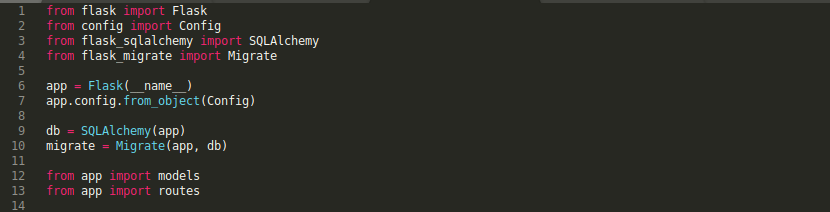
\includegraphics[width=14cm]{back_captures/init_file}
	\caption{\textit{{\_}{\_}init{\_}{\_}.py} file}
	\label{fig:init_file}
\end{figure}

The \textit{routes.py} file is where the different calls to the server are defined (Figure \ref{fig:routes_file}), among which we can find "/recognise{\_}me" to identify a student using a photo, "/next{\_}class" to obtain the next class of a student using the ID number related to that student, and "/map" to obtain a map image with a path from the origin point to the destination point. In order to carry out these calls, the rest of the modules of the server (stored in the "utils" folder) are called. 

\begin{figure}[!ht]
	\centering
	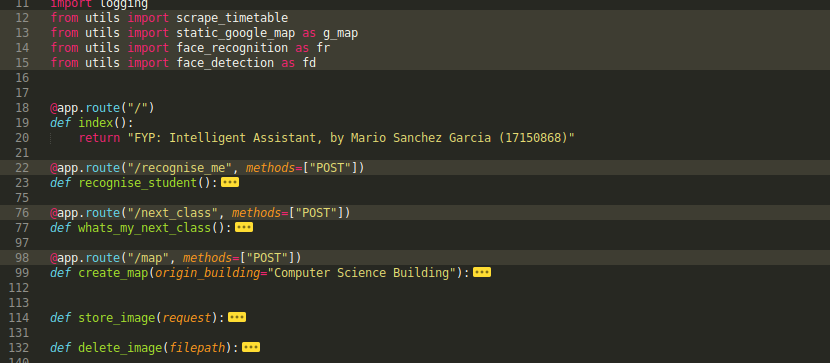
\includegraphics[width=14cm]{back_captures/routes_file}
	\caption{Structure of the \textit{routes.py} file}
	\label{fig:routes_file}
\end{figure}

	\subsection{Face detection module}
	\label{subsec:face_det}
	This section refers to the \textit{face{\_}detection.py} file. It has two important functions called \textit{detect{\_}face} and \textit{lfw{\_}detect{\_}face}. The first is used to perform the face detection for the server, using a single file, while the second has been only used during the training of the network with the \gls{lfw} dataset, being adapted to the particular file structure of the dataset. Only \textit{face{\_}detection} (Figure \ref{fig:detect_face_function}) will be explained here but as both functions work pretty similar, the same explanation can be applied to the other one.

	\begin{figure}[!ht]
		\centering
		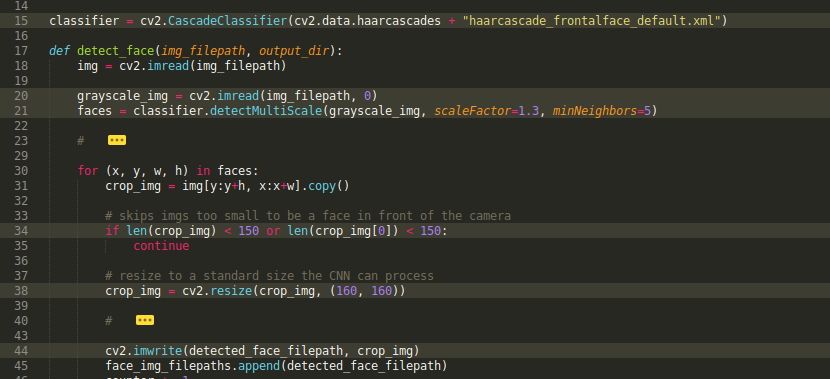
\includegraphics[width=14cm]{back_captures/detect_face}
		\caption{\textit{detect{\_}face} function}
		\label{fig:detect_face_function}
	\end{figure}

	First, from the OpenCV library the the classifier "haarcascade{\_}frontface{\_}default" is loaded, which applies the previously explained Viola-Jones method using Haar features (Section \ref{subsec:face_detec_techniques}). The image is loaded in grayscale , as this method work with the pixel intensities, not with the colour channels. Using the classifier, the coordinates of the detected faces are obtained and stored in the array \textit{faces}. 

	The detected faces that are smaller than 150 pixels are discarded. The reason after this is that it has been assumed that the user is always near the camera when the photo is taken, so if a small face is detected, it would be either another person in the background or a false positive.

	The face image is finally resized to a square of 160 pixels because the \gls{cnn} cannot accept smaller images. During the convolution process, the pooling makes the image smaller in each step, so if the image has less than 160x160 pixels, in one of these steps it will not be possible to apply the pooling.

	\subsection{Face recognition module}
	\label{subsec:face_recog}
	The \textit{train{\_}classifier.py} has been chosen to be explained here because its main role in the face recognition. Nevertheless, as it has been shown in the component diagram (Figure \ref{fig:back_comp_diagram}), many others files contribute to make it possible.

	This file is used by itself to train and evaluate the \gls{cnn} (\textit{main} function, Figure \ref{fig:train_classifier_main}), and as a library to get the prediction of who is the student in front of the camera (\textit{get{\_}prediction} function, Figure \ref{fig:get_pred_function}). 

	\begin{figure}[!ht]
		\centering
		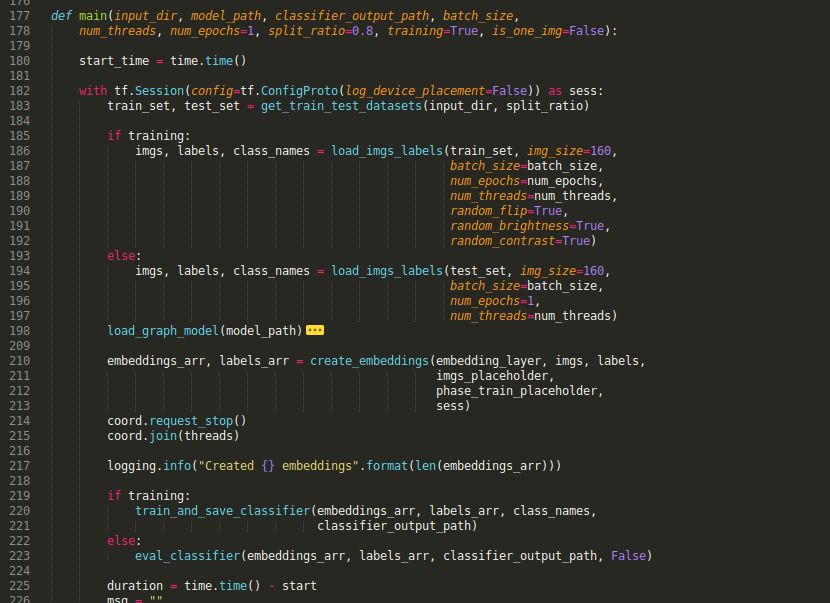
\includegraphics[width=14cm]{back_captures/train_class_main}
		\caption{\textit{main} function from \textit{train{\_}classifier.py}}
		\label{fig:train_classifier_main}
	\end{figure}

	The \textit{main} function starts creating a Tensorflow session (line 182) to encapsulate the environment in which the tensors are evaluated. Then, the images from the \gls{lfw} dataset are loaded and splitted into the train and test sets (line 183). Internally, Tensorflow does not use the class names (student IDs, in this case) to identify the person that appears in the image. Instead, it uses an integer known as "label". These labels are created when the images are loaded, asigning them label values starting from 0.  

	Image files, labels and class names are loaded from the train or the test set, depending on whether it is training or evaluation. During the training, the pool of images is increased by applying random flips and slight brightness and contrast changes to the original images (lines 190-192). Onthe other hand, during the evaluation, the number of \glspl{epoch} is fixed to 1 (line 196) because the output of every epoch would be the same, as the classifier does not change.

	Now is when the pre-trained model (Inception Resnet v1) is loaded. Using this model, the \glspl{embedding} are extracted from the image, distributing the work among the defined number of threads (line 210). Once the embeddings have been created, they are used to train a SVC classifier and save it later to a .pkl file (line 220). This same classifier is used to evaluate how similar are the recently extracted embeddings to the embeddings of the students with whom it was trained in first place (line 223).

	The \textit{get{\_}prediction} (Figure \ref{fig:get_pred_function}) function is pretty similar to the \textit{main} function, but instead of using a full dataset, the input is a single image. It was created specifically for the interaction between the Raspberry Pi and the server, evaluating the received image with the classifier. In this case, the ID number of the student with the best probability and the value of this probability is returned, so the server will be able to evaluate if it is high enough to assure that the student was in fact recognised.

	\begin{figure}[!ht]
		\centering
		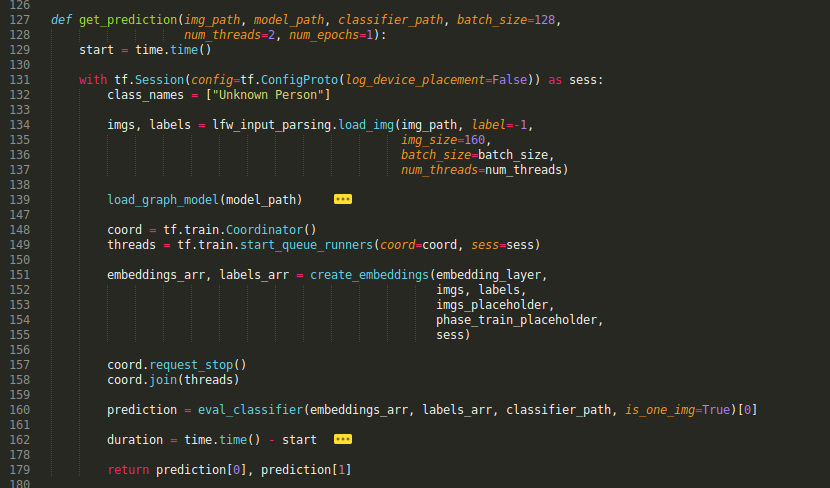
\includegraphics[width=14cm]{back_captures/get_pred_function}
		\caption{\textit{get{\_}prediction} function from \textit{train{\_}classifier.py}}
		\label{fig:get_pred_function}
	\end{figure}

	\subsection{Web scraping module}
	\label{subsec:scraping_module}
	This module is contained in \textit{scrape{\_}timetable.py}. The only available function in this file, \textit{get{\_}week{\_}timetable} (Figure \ref{fig:get_timetable_function}), is called from the server in order to get the full timetable of the student. Is in the server itself where it is evaluated if the student has more classes using this week timetable.

	\begin{figure}[!ht]
		\centering
		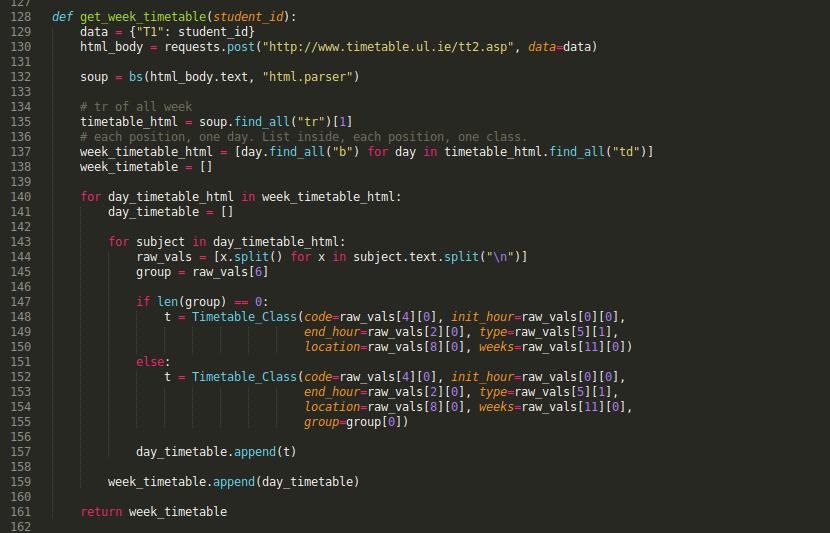
\includegraphics[width=14cm]{back_captures/week_timetable_function}
		\caption{\textit{get{\_}week{\_}timetable} function}
		\label{fig:get_timetable_function}
	\end{figure}

	First, the student ID is used to log into the website by introduce it into the field "T1" (lines 129-130), that corresponds with the input tag in the HTML. The response, that contains the timetable page, is stored and the Beautiful Soup library is used to parse it to a format it can work with (line 132). The timetable is always inside the second "$<tr>$" tag (line 135) and inside it, the days are inside $<td>$ tags and the classes into $<b>$ tags (line 137). 

	The tags are deleted and the text is splitted by the whitespace character (line 144). As the structure is always the same, the values always correspond for the same fields. These values are used to create a \textit{Timetable} object, which is defined in the same file. 

	In the \textit{{\_}{\_}init{\_}{\_}} of the object (Figure \ref{fig:timetable_object}), the different parse methods (lines 87, 103, 123) are called to store the parameters as attributes of the object. The parse methods, using the \textit{re} library, compile regular expressions and obtain the actual values from the raw input (line 124). As the name of the module is not provided in the timetable, another request is necessary (line 77). Following a similar process, the Beautiful Soup library is used again to obtain the module name from "timetable.ul.ie/tt{\_}moduledetails.asp".

	\begin{figure}[!ht]
		\centering
		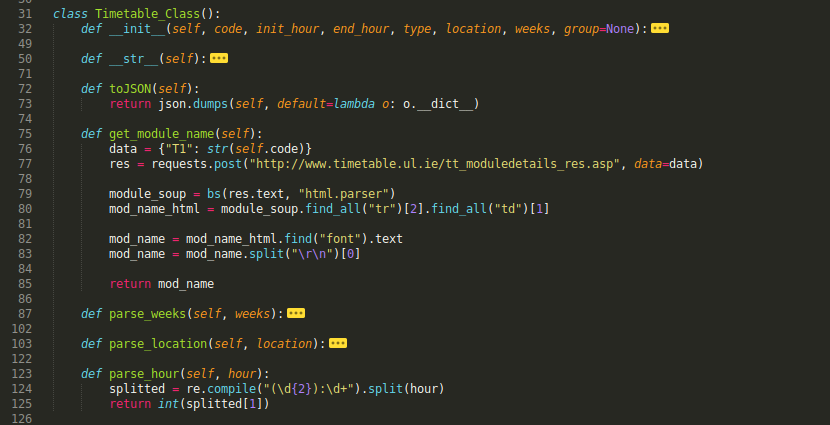
\includegraphics[width=14cm]{back_captures/timetable_object}
		\caption{\textit{Timetable} object}
		\label{fig:timetable_object}
	\end{figure}
	
	\subsection{Map module}
	\label{subsec:map_module}
	This section refers to the \textit{static{\_}google{\_}map.py} file. Here, the Google Maps API is used to obtain a map image with a pin at the origin point, another pin at the destination point and a path that connects them. The way to use this API is to send a GET HTML request to a certain url (Figure \ref{fig:get_map_url_function}, line 42), including the parameters of the map and the Google developer key in it. 

	\begin{figure}[!ht]
		\centering
		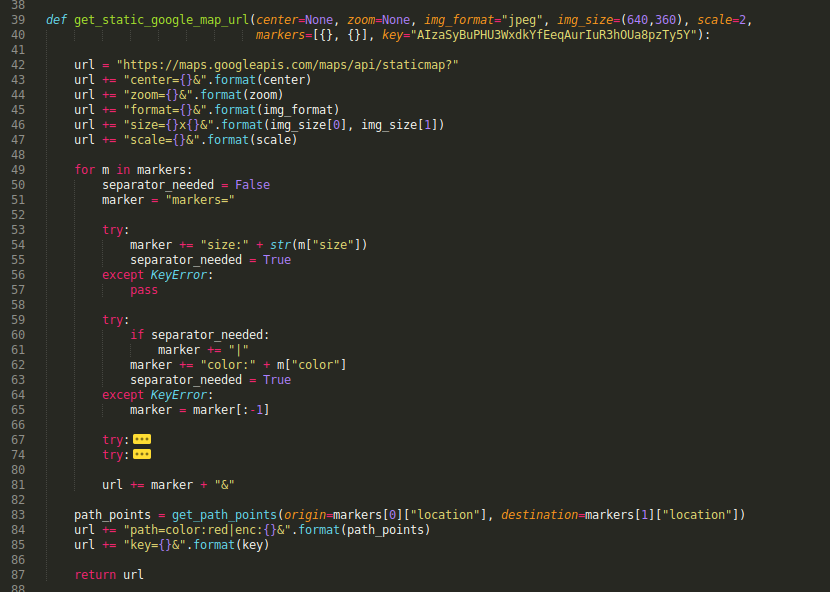
\includegraphics[width=14cm]{back_captures/get_map_url}
		\caption{\textit{get{\_}static{\_}google{\_}map{\_}url} function}
		\label{fig:get_map_url_function}
	\end{figure}

	The function \textit{get{\_}static{\_}google{\_}map{\_}url} generates this url concatenating the parameters in the format of a GET request. Although the image must have a \gls{720p} resolution, the standard users of the API have a maximum image size of 640x360, so the option "scale" is also used to resize it (line 39). If the path is defined with just the locations of the origin and the destination, the result is a straight line connecting both points. In order to obtain a real path, the Google Directions API is also used in the function \textit{get{\_}path{\_}points} (line 83).

	Once the url is created, \textit{get{\_}map{\_}image}, which is the function used by the server, sends the GET request and returns the image.
	


%████████╗███████╗███████╗████████╗██╗███╗   ██╗ ██████╗ 
%╚══██╔══╝██╔════╝██╔════╝╚══██╔══╝██║████╗  ██║██╔════╝ 
%   ██║   █████╗  ███████╗   ██║   ██║██╔██╗ ██║██║  ███╗
%   ██║   ██╔══╝  ╚════██║   ██║   ██║██║╚██╗██║██║   ██║
%   ██║   ███████╗███████║   ██║   ██║██║ ╚████║╚██████╔╝
%   ╚═╝   ╚══════╝╚══════╝   ╚═╝   ╚═╝╚═╝  ╚═══╝ ╚═════╝ 
                                                    
\section{Testing}
\label{sec:testing}
Two approaches are possible to perform the testing: automated, where a set of unit tests are executed to obtain a "passed"/"failed" answer, and manual testing, where is a human who applies the tests to the system. The automated testing on a GUI is actually possible (e.g. \cite{maveryx_testing}), but the manual testing was finally chosen because its simplicity. The results of this testing are displayed in following tables (\ref{table:fun_1_req_validation}, \ref{table:fun_2_req_validation}, \ref{table:non_fun_req_validation}), where the requirements have been validated to verify the proper operation of the system.

\clearpage

\begin{table}[p]
	\centering
	\resizebox{\textwidth}{!}
	{
    \begin{tabular}{| C{2cm} | C{3cm} | L{9cm} |}
	    \hline
	    \textbf{ID} & \textbf{Satisfied} & \multicolumn{1}{c|}{\textbf{Notes}} \\
	    \hline
	    FR{\_}01 & \checkmark & Architectural requirement. See \ref{sec:architecture}. \\
	    \hline
	    FR{\_}02 & \checkmark & Architectural requirement. See \ref{sec:architecture}. \\
	    \hline
	    FR{\_}03 & \checkmark & Architectural requirement. See \ref{sec:architecture}. \\
	    \hline
	    FR{\_}04 & \checkmark & Architectural requirement. See \ref{sec:architecture}. \\
	    \hline
	    FR{\_}05 & \xmark & Not satisfied in the Loading window. As an optional requirement, used mostly during the development of the app, it is an acceptable behaviour. \\
	    \hline
	    FR{\_}06 & \checkmark & Showing the focus (blue icons), disabled button (gray icons) and waiting for server response (yellow icons). \\
	    \hline
	    FR{\_}07 & \checkmark & Architectural requirement. See \ref{sec:architecture}. \\
	    \hline
	    FR{\_}08 & \xmark & Not satisfied in the Loading window, but within the expected behaviour. See FR{\_}09.  \\
	    \hline
	    FR{\_}09 & \checkmark & Included in Loading window. See \ref{sec:scenario} \\
	    \hline
	    FR{\_}10 & \checkmark & Included in Preview window. See \ref{sec:scenario} \\
	    \hline
	    FR{\_}11 & \checkmark & Included in Preview window. See \ref{sec:scenario} \\
	    \hline
	    FR{\_}12 & \checkmark & Included in Preview window. See \ref{sec:scenario} \\
	    \hline
	    FR{\_}13 & \checkmark & Included in Snapshot window. See \ref{sec:scenario} \\
	    \hline
	    FR{\_}14 & \checkmark & \multicolumn{1}{c|}{-} \\
	    \hline
	    FR{\_}15 & \checkmark & Included in \textit{routes.py}, see Figure \ref{fig:routes_file}. \\
	    \hline
	    FR{\_}16 & \checkmark & Loading window. See \ref{sec:scenario}  \\
	    \hline
	    FR{\_}17 & \checkmark & \multicolumn{1}{c|}{-} \\
	    \hline
	    FR{\_}18 & \checkmark & \multicolumn{1}{c|}{-} \\
	    \hline
	    FR{\_}19 & \checkmark & Face detection module. See \ref{subsec:face_det} \\
	    \hline
	    FR{\_}20 & \checkmark & Error window. See \ref{sec:scenario} \\
	    \hline
	\end{tabular}	    
	}
	\caption{Functional Requirements (1-20) validation}
    \label{table:fun_1_req_validation}
\end{table}

\clearpage

\begin{table}[p]
	\centering
	\resizebox{\textwidth}{!}
	{
    \begin{tabular}{| C{2cm} | C{3cm} | L{9cm} |}
	    \hline
	    \textbf{ID} & \textbf{Satisfied} & \multicolumn{1}{c|}{\textbf{Notes}} \\
	    \hline
	    FR{\_}21 & \checkmark & Face detection module. See \ref{subsec:face_det} \\
	    \hline
	    FR{\_}22 & \checkmark & Error window. See \ref{sec:scenario} \\
	    \hline
	    FR{\_}23 & \checkmark & File \textit{reset{\_}db.py}. See \ref{subsec:sql_alchemy} \\
	    \hline
	    FR{\_}24 & \checkmark & Response of the server for the face recognition process. See \ref{sec:scenario} \\
	    \hline
	    FR{\_}25 & \checkmark & Timetable window. See \ref{sec:scenario} \\
	    \hline
	    FR{\_}26 & \checkmark & Included in \textit{routes.py}, see Figure \ref{fig:routes_file}. \\
	    \hline
	    FR{\_}27 & \checkmark & Included in \textit{scrape{\_}timetable.py}, see \ref{subsec:scraping_module}. \\
	    \hline
	    FR{\_}28 & \checkmark & Included in \textit{scrape{\_}timetable.py}, see \ref{subsec:scraping_module}. \\
	    \hline
	    FR{\_}29 & \xmark & Not all the information was included in the response because it is not shown in the application, so it is not necessary to send it back. \\
	    \hline
	    FR{\_}30 & \checkmark & No More Classes window. See \ref{sec:scenario} \\
	    \hline
	    FR{\_}31 & \checkmark & Timetable window. See \ref{sec:scenario} \\
	    \hline
	    FR{\_}32 & \checkmark & Included in \textit{routes.py}, see Figure \ref{fig:routes_file}. \\
	    \hline
	    FR{\_}33 & \checkmark & Map module. See \ref{subsec:map_module} \\
	    \hline
	    FR{\_}34 & \checkmark & Map module. See \ref{subsec:map_module} \\
	    \hline
	    FR{\_}35 & \checkmark & Map module. See \ref{subsec:map_module} \\
	    \hline
	    FR{\_}36 & \checkmark & Map window. See \ref{subsec:map_window} \\
	    \hline
	    FR{\_}37 & \checkmark & Lateral menu of the Home window. See \ref{sec:scenario} \\
	    \hline
	    FR{\_}38 & \checkmark & Lateral menu of the Home window. See \ref{sec:scenario} \\
	    \hline
	    FR{\_}39 & \checkmark & Lateral menu of the Home window. See \ref{sec:scenario} \\
	    \hline
	\end{tabular}	    
	}
	\caption{Functional Requirements (21-39) validation}
    \label{table:fun_2_req_validation}
\end{table}

\clearpage


\begin{table}[!ht]
	\centering
	\resizebox{\textwidth}{!}
	{
    \begin{tabular}{| C{2cm} | C{3cm} | L{9cm} |}
	    \hline
	    \textbf{ID} & \textbf{Satisfied} & \multicolumn{1}{c|}{\textbf{Notes}} \\
	    \hline
	    NFR{\_}01 & \checkmark & Included in the Flask server. See \ref{sec:techs}. \\
	    \hline
	    NFR{\_}02 & \checkmark & Included in the Flask server. See \ref{sec:techs}. \\
	    \hline
	    NFR{\_}03 & \checkmark & Setup of the project. See \ref{sec:scenario}. \\
	    \hline
	    NFR{\_}04 & \checkmark & Included in the attributes of the root window. See \ref{sec:front_end}. \\
	    \hline
	    NFR{\_}05 & \checkmark & \multicolumn{1}{c|}{-} \\
	    \hline
	    NFR{\_}06 & \checkmark & Lateral menu. See \ref{sec:scenario}. \\
	    \hline
	    NFR{\_}07 & \checkmark & Lateral menu. See \ref{sec:scenario}. \\
	    \hline
	    NFR{\_}08 & \checkmark & \multicolumn{1}{c|}{-} \\
	    \hline
	    NFR{\_}09 & \checkmark & Face detection face recognition modules. See \ref{subsec:face_det} and \ref{subsec:face_recog}. \\
	    \hline
	    NFR{\_}10 & \checkmark & Web scraping module. See \ref{subsec:scraping_module}. \\
	    \hline
	    NFR{\_}11 & \checkmark & Map module. See \ref{subsec:map_module}. \\
	    \hline
	    NFR{\_}12 & \checkmark & Face recognition module. See \ref{subsec:face_recog}.  \\
	    \hline
	    NFR{\_}13 & \checkmark & See \ref{sec:scenario}. \\
	    \hline
	    NFR{\_}14 & \checkmark & \multicolumn{1}{c|}{-} \\
	    \hline
	    NFR{\_}15 & \checkmark & \multicolumn{1}{c|}{-} \\
	    \hline
	\end{tabular}	    
	}
	\caption{Non-Functional Requirements validation}
    \label{table:non_fun_req_validation}
\end{table}

\clearpage


%██╗███╗   ███╗██████╗ ██╗     ███████╗███╗   ███╗       ██╗███████╗███████╗██╗   ██╗███████╗███████╗
%██║████╗ ████║██╔══██╗██║     ██╔════╝████╗ ████║       ██║██╔════╝██╔════╝██║   ██║██╔════╝██╔════╝
%██║██╔████╔██║██████╔╝██║     █████╗  ██╔████╔██║       ██║███████╗███████╗██║   ██║█████╗  ███████╗
%██║██║╚██╔╝██║██╔═══╝ ██║     ██╔══╝  ██║╚██╔╝██║       ██║╚════██║╚════██║██║   ██║██╔══╝  ╚════██║
%██║██║ ╚═╝ ██║██║     ███████╗███████╗██║ ╚═╝ ██║██╗    ██║███████║███████║╚██████╔╝███████╗███████║
%╚═╝╚═╝     ╚═╝╚═╝     ╚══════╝╚══════╝╚═╝     ╚═╝╚═╝    ╚═╝╚══════╝╚══════╝ ╚═════╝ ╚══════╝╚══════╝
                                                                                                    
\section{Implementation issues}
Many issues were found during the development of the system and, in order to help other developers who use the same technologies as in this project, this section will explain how some of these issues were solved.

The first big problem developing the system came while OpenCV was being installed in the Raspberry Pi. As said before (Section \ref{subsec:opencv}), OpenCV is not installed by default for the version 3 of Python. The problem is that the command \textit{sudo apt-get install python-opencv} to install it from pre-built binaries does not work, because the Raspberry Pi architecture is not supported. 

The only option left was to build it from the source code. Following the tutorial also mentioned before, the Raspberry Pi compiled the source code, but it targeted Python 2.x instead of Python 3, being in the same situation as at the beginning. After inspecting the logs of the compilation process, an ImportError was found: the library depency "atlas" was not installed. Once it was installed, the compilation process was repeated and OpenCV was finally available for Python3.

Other issue was found while developing the application \gls{gui}. Many icons and images have been used in the \gls{gui}, some because they were necessary and others for aesthetic reasons. The process followed to load them was first read image file using OpenCV, resize it as necessary, change the colour space to RGB (OpenCV uses BGR), create a PhotoImage object and link it to the widget where the image was going to be displayed. However, the image was not displayed. 

From \cite{tkinter_images_double_ref}:

\say{The problem is that the Tkinter/Tk interface doesn’t handle references to Image objects properly; the Tk widget will hold a reference to the internal object, but Tkinter does not. When Python’s garbage collector discards the Tkinter object, Tkinter tells Tk to release the image. But since the image is in use by a widget, Tk doesn’t destroy it. Not completely. It just blanks the image, making it completely transparent…}

The solution to this problem was to link the image twice, first to the "image" attibute and then to the image object of the widget.

The third and last issue that is going to be explained here is related to how an image is sent in a HTML message using JSON. It was thought at first to create a dictionary to store a key "image" with the binary data of the image as value. However, after running the script, it was discovered that JSON does not support binary data. Is because of this reason that it was decided to encode the binary data in \gls{base64} on one side of the communication and decode it on the other, obtaining the image as if it was just read from the file.

\section{Summary of the implementation}
In order to measure the size of the system and the effort involved in its development, it has been chosen as metric the lines of code (\glspl{loc}). We can find the \glspl{loc} of each file in the Table \ref{table:loc_per_file}, having at the end the total amount of \glspl{loc} of the system.

\begin{table}[!ht]
	\centering
    \begin{tabular}{| C{2cm} | C{3cm}  L{5cm} | R{2cm} |}
	    \hline
	    \multicolumn{3}{|c|}{\textbf{FILE}}	&	\multicolumn{1}{c|}{\textbf{\glspl{loc}}} \\
	    \hline
	    \multirow{2}{*}{Front End}  
	    	& \multirow{2}{*}{Application} 	& \multicolumn{1}{|l|}{app.py} 	&	978 \\ \cline{3-4}

	    	& &					 \multicolumn{1}{r|}	{\textit{Subtotal}}	& 	\textit{978}	\\ 
	    \hline
%	    \multicolumn{2}{|c}{Front End}	
%	    		& \multicolumn{1}{|l|}{app.py} 							&	978		\\
%	    \hline
	    \multirow{14}{*}{Back End}
	    	& \multirow{7}{*}{Server} 	
	    		& \multicolumn{1}{|l|}{server.py} 						& 	  8 	\\ \cline{3-4}
	    	&	& \multicolumn{1}{|l|}{{\_}{\_}init{\_}{\_}.py} 		& 	 13 	\\ \cline{3-4}
	    	&	& \multicolumn{1}{|l|}{config.py} 						& 	 14 	\\ \cline{3-4}
	    	&	& \multicolumn{1}{|l|}{models.py} 						& 	  8 	\\ \cline{3-4}
	    	&	& \multicolumn{1}{|l|}{reset{\_}db.py} 					& 	 35 	\\ \cline{3-4}
	    	&	& \multicolumn{1}{|l|}{routes.py} 						& 	140 	\\ \cline{3-4}

	    	&	& \multicolumn{1}{r|}				{\textit{Subtotal}}	& 	\textit{218} 	\\ 
	    	
	    	\cline{2-4}
	    	
	    	& \multirow{7}{*}{Utilities} 	
	    		& \multicolumn{1}{|l|}{face{\_}detection.py} 			& 	158		\\ \cline{3-4}
	    	&	& \multicolumn{1}{|l|}{scrape{\_}timetable.py} 			& 	170		\\ \cline{3-4}
	    	&	& \multicolumn{1}{|l|}{static{\_}google{\_}map.py} 		& 	125		\\ \cline{3-4}
	    	&	& \multicolumn{1}{|l|}{face{\_}recognition.py} 			& 	  8		\\ \cline{3-4}
	    	&	& \multicolumn{1}{|l|}{lfw{\_}input{\_}parsing.py} 		& 	130		\\ \cline{3-4}
	    	&	& \multicolumn{1}{|l|}{train{\_}classifier.py} 			& 	262		\\ \cline{3-4}

	    	&	& \multicolumn{1}{r|}				{\textit{Subtotal}}	& 	\textit{853}	\\ 
	    \hline
	    \multicolumn{3}{|r|}								{\textbf{TOTAL}}			&  \textbf{2,049} \\ 
	    \hline
	\end{tabular}
	\caption{\glspl{loc} per file and total \glspl{loc} of the project}
    \label{table:loc_per_file}
\end{table}



%███████╗ ██████╗ ███████╗████████╗     ██████╗ ██╗   ██╗ █████╗ ██╗     ██╗████████╗██╗   ██╗
%██╔════╝██╔═══██╗██╔════╝╚══██╔══╝    ██╔═══██╗██║   ██║██╔══██╗██║     ██║╚══██╔══╝╚██╗ ██╔╝
%███████╗██║   ██║█████╗     ██║       ██║   ██║██║   ██║███████║██║     ██║   ██║    ╚████╔╝ 
%╚════██║██║   ██║██╔══╝     ██║       ██║▄▄ ██║██║   ██║██╔══██║██║     ██║   ██║     ╚██╔╝  
%███████║╚██████╔╝██║        ██║██╗    ╚██████╔╝╚██████╔╝██║  ██║███████╗██║   ██║      ██║   
%╚══════╝ ╚═════╝ ╚═╝        ╚═╝╚═╝     ╚══▀▀═╝  ╚═════╝ ╚═╝  ╚═╝╚══════╝╚═╝   ╚═╝      ╚═╝   
                                                                                             
\section{Software Quality}
Software Quality methods help in the development of an application, allowing the client's ideas to be interpreted in the most reliable possible way, so they will be reflected and included in the final product. The development group of the project must be strict when following these methods in order to obtain the best output. For big projects, where several people work together in the development, they help both in the communication client-developer and the internal communication within the work groups.

However, the numerous rules that must be followed for this method to be effective make that the strictly applicattion of such methods on a project of the scale of a FYP, in which only one person is client and developer at the same time, may not be advisable, investing a time in the process that will not be rewarded with notorious results. However, some notions of Software Quality have been followed in the development of the project, collecting the ideas about the project into requirements (\ref{sec:requirements}) and after checking if they were finally included in the final result (\ref{sec:testing}).


